\documentclass[UTF8,fontset=fandol,oneside]{ctexbook}

\usepackage{amsmath,amssymb,bm,mathtools}
\usepackage[a4paper,left=30mm,right=30mm,top=30mm,bottom=30mm,headheight=16pt,headsep=8mm]{geometry}
\usepackage{graphicx}
\usepackage{booktabs}
\usepackage{microtype}
\usepackage[hidelinks]{hyperref}
\usepackage{caption}
\usepackage{fancyhdr}

\graphicspath{{../content/images/}}
\providecommand{\pmb}[1]{\boldsymbol{#1}}
\setcounter{secnumdepth}{3}
\setcounter{tocdepth}{3}
\allowdisplaybreaks
\setlength{\emergencystretch}{3em}
\pagestyle{fancy}
\fancyhf{}
\fancyhead[C]{\nouppercase{\leftmark}}
\fancyfoot[C]{\thepage}
\renewcommand{\headrulewidth}{0.4pt}
\renewcommand{\chaptermark}[1]{\markboth{第\thechapter 章\quad #1}{}}
\fancypagestyle{plain}{%
  \fancyhf{}%
  \fancyhead[C]{\nouppercase{\leftmark}}%
  \fancyfoot[C]{\thepage}%
  \renewcommand{\headrulewidth}{0.4pt}%
}

\hypersetup{
  pdftitle={SLAM Handbook：从定位与建图到空间智能（第1、2章中文翻译）},
  pdfauthor={SLAM Handbook 中文翻译项目}
}

\begin{document}

\frontmatter
\title{SLAM Handbook\\从定位与建图到空间智能}
\author{第 1、2 章中文翻译}
\date{\today}
\maketitle

\chapter*{版权与翻译说明}
\addcontentsline{toc}{chapter}{版权与翻译说明}

本书原著由 Luca Carlone、Ayoung Kim、Timothy Barfoot、Daniel Cremers 和 Frank Dellaert 编辑，\textcopyright{} Cambridge University Press。

本 PDF 是 SLAM Handbook 第 1、2 章的中文翻译排版版本。原作者、编辑、出版方及原项目的版权和署名信息均予以保留。中文翻译内容仅在获得相应授权的范围内公开使用。

\tableofcontents

\mainmatter
\chapter{SLAM 的因子图}

\textbf{作者：} Frank Dellaert、Michael Kaess、Timothy Barfoot

本章介绍因子图，并在高斯先验和高斯测量噪声的条件下，建立最大后验（maximum a posteriori，MAP）推断与最小二乘之间的联系。我们关注 SLAM 后端，即前端已经提取测量并完成数据关联之后的部分。首先，我们使用因子图对 SLAM 问题进行可视化（第 1.1 节）；随后说明 MAP 推断如何导出最小二乘优化（第 1.2 节）。接着讨论线性优化（第 1.3 节）和非线性优化（第 1.4 节）的求解方法，并进一步明确稀疏性、因子图和贝叶斯网络之间的联系（第 1.5 节）。然后介绍变量消元算法及其图模型解释（第 1.6 节），最后据此构建贝叶斯树以及增量平滑与建图（iSAM）算法（第 1.7 节）。本章最后讨论延伸阅读与近期趋势（第 1.8 节）。

\section*{历史注记}
\addcontentsline{toc}{section}{历史注记}

SLAM 的平滑方法不仅考虑机器人当前时刻的位置，还考虑截至当前时刻的完整机器人轨迹。许多作者只研究机器人轨迹的平滑问题 \textsuperscript{[172, 701, 700, 420, 594, 312]}，这类方法如今称为\textbf{基于位姿的 SLAM}（pose-based SLAM）。它尤其适用于激光测距仪等传感器，因为这类传感器会在相邻机器人位姿之间产生两两约束。

更一般地，可以考虑完整 SLAM 问题 \textsuperscript{[1088]}，即在最优意义下，同时估计全部传感器位姿以及环境中所有特征的参数。从计算角度看，这种基于优化的平滑方法具有明显优势：（a）与基于滤波的协方差矩阵或信息矩阵不同，后两者都会随时间推移逐渐变成完全稠密的矩阵 \textsuperscript{[849, 1087]}，而平滑对应的信息矩阵保持稀疏；（b）在典型建图场景中（也就是机器人并非反复穿行于一个很小的环境），该矩阵能够更紧凑地表示地图协方差结构。由此，在 2000—2005 年间，大量工作开始将这些思想应用于 SLAM \textsuperscript{[287, 340, 339, 1088]}。

基于平方根的平滑与建图（square-root smoothing and mapping，SAM），也称为“因子图方法”，是在 \textsuperscript{[249, 254]} 中提出的，其依据是：信息矩阵或测量雅可比矩阵可以分别通过稀疏 Cholesky 分解或 QR 分解进行高效分解。这样便得到一个平方根信息矩阵，可立即用于求取最优机器人轨迹和地图。在序贯估计文献中，对信息矩阵进行分解被称为\textbf{平方根信息滤波}（square-root information filtering，SRIF）；该方法于 1969 年为 JPL 的水手 10 号（Mariner 10）金星探测任务而发展 \textsuperscript{[83]}。使用平方根能够得到更加准确、稳定的算法。引用 Maybeck \textsuperscript{[742]} 的话说：“许多实践者以充分的逻辑依据主张：平方根滤波器应始终优先于标准的卡尔曼滤波递推。”

下面我们将详细讨论：因子图为何是表示 SLAM 问题固有稀疏性的自然工具；将矩阵进行（稀疏）分解并得到矩阵平方根为何是求解这类问题的核心；以及这些内容最终如何与更一般的变量消元算法联系起来。本章的大部分内容是 Dellaert 等人 \textsuperscript{[255]} 长篇文章的压缩版。

\section{用因子图直观表示 SLAM}

本节首先通过一个玩具示例及其因子图表示，引入因子图，直观展示 SLAM 问题的稀疏性。随后说明多种不同形式的 SLAM 都可以采用这种表示，即使面对更大规模的问题，其稀疏结构也通常一目了然。

\subsection{一个玩具示例}

我们先考察一个简单的 SLAM 场景，以说明如何构造因子图。图 1.1 给出了该问题结构的示意图。机器人依次经过三个位姿 ${ \mathbf { \mathit { p } } } _ { 1 }$、${ \mathbf { \mathit { p } } } _ { 2 }$ 和 $p_3$，并对两个路标 $\ell_1$ 和 $\ell_2$ 进行方位观测。为了将解锚定在空间中，假设在第一个位姿 ${ \pmb p }_1$ 上还有一个绝对位置/方向测量。没有这一测量，就无法获得绝对位置的信息，因为方位测量都是相对的。\textsuperscript{1}

\begin{figure}[htbp]
\centering
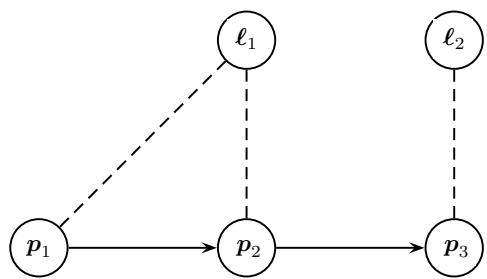
\includegraphics[width=\linewidth]{7f2cd7879950afca0abfe3a2c35a1a703e4d6c8e28ee44484e2aef43386318b3.jpg}
\caption{图 1.1 三个位姿和两个路标构成的玩具同步定位与建图（SLAM）示例。图中用箭头示意机器人运动，用虚线表示方位测量。}
\label{fig:7f2cd7879950afca0abfe3a2c35a1a703e4d6c8e28ee44484e2aef43386318b3}
\end{figure}

由于测量存在不确定性，我们不可能恢复世界的真实状态，但可以得到一个关于测量能够推断出的内容的概率描述。在贝叶斯概率框架中，我们使用概率论的语言，为不确定事件赋予主观的可信程度。具体而言，对未知变量 $\pmb x$ 定义概率密度函数（probability density function，PDF）$p(\pmb x)$。PDF 是满足下式的非负函数：

\begin{equation}
\int p (\boldsymbol {x}) \,\mathrm{d} \boldsymbol {x} = 1,\tag{1.1}
\end{equation}

这就是全概率公理。在图 1.1 的简单示例中，状态 $\pmb x$ 为

\begin{equation}
\boldsymbol {x} = \left[ \begin{array}{c} \boldsymbol {p} _ {1} \\ \boldsymbol {p} _ {2} \\ \boldsymbol {p} _ {3} \\ \boldsymbol {\ell} _ {1} \\ \boldsymbol {\ell} _ {2} \end{array} \right],\tag{1.2}
\end{equation}

也就是将各个未知量依次堆叠起来。

在 SLAM 中，给定一组观测测量 $\pmb z$ 后，我们希望刻画关于未知量 $\pmb x$ 的知识；在本例中，未知量包括机器人位姿和未知的路标位置。用贝叶斯概率的语言，这就是条件密度或后验密度：

\begin{equation}
p (\boldsymbol {x} | \boldsymbol {z}),\tag{1.3}
\end{equation}

获得这样的描述称为\textbf{概率推断}。在此之前，必须先为感兴趣的变量以及它们如何产生（不确定的）测量指定概率模型。这正是概率图模型发挥作用的地方。

概率图模型利用概率分布中的结构，为复杂概率密度提供紧凑的描述机制 \textsuperscript{[592]}。贝叶斯网络可能是最广为人知的图模型：它由变量节点组成，每个变量节点都关联一个先验概率密度或条件概率密度。图 1.2 展示了图 1.1 玩具示例对应的贝叶斯网络，其中明确给出了依赖于第一个位姿 $\pmb p_1$ 的初始测量 $z_1$，以及 $z_2\ldots z_4$ 四个方位测量，每个测量都同时与一个位姿和一个路标相关。按照惯例，贝叶斯网络中已知量用方形节点表示，如图所示。不过，贝叶斯网络虽然非常适合建模，下面我们还要引入另一种更适合优化的图模型；它只关注问题中的未知变量。

\begin{figure}[htbp]
\centering
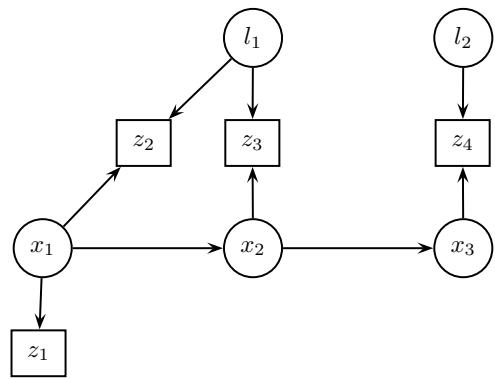
\includegraphics[width=\linewidth]{de0dd895a761a6a8ef2799623bc1231feeeca13f4f5f7a71c2097acf985dfe2a.jpg}
\caption{图 1.2 图 1.1 示例对应的贝叶斯网络，其中将已知测量 $z_1\ldots z_4$ 明确表示为方形节点。}
\label{fig:de0dd895a761a6a8ef2799623bc1231feeeca13f4f5f7a71c2097acf985dfe2a}
\end{figure}

\subsection{因子图视角}

由于局部性，高维概率密度通常可以分解为许多因子的乘积，每个因子只是定义在一个更小域上的概率密度。因子图是一类概率图模型，它允许我们将任意密度表示为因子的乘积。

为了说明因子图的动机，考虑如何对上述玩具 SLAM 示例执行推断。根据贝叶斯定律，后验 $p(\pmb x|\pmb z)$（式 1.3）可写为 $p(\pmb x|\pmb z) \propto p(\pmb z|\pmb x)p(\pmb x)$，于是

\begin{equation}
p (\pmb {x} | \pmb {z}) \propto p (\pmb {p} _ {1}) p (\pmb {p} _ {2} | \pmb {p} _ {1}) p (\pmb {p} _ {3} | \pmb {p} _ {2})\tag{1.4a}
\end{equation}

\begin{equation}
\times p (\pmb {\ell} _ {1}) p (\pmb {\ell} _ {2})\tag{1.4b}
\end{equation}

\begin{equation}
\times p (\boldsymbol {z} _ {1} | \boldsymbol {p} _ {1})\tag{1.4c}
\end{equation}

\begin{equation}
\times p (\boldsymbol {z} _ {2} | \boldsymbol {p} _ {1}, \ell_ {1}) p (\boldsymbol {z} _ {3} | \boldsymbol {p} _ {2}, \ell_ {1}) p (\boldsymbol {z} _ {4} | \boldsymbol {p} _ {3}, \ell_ {2}).\tag{1.4d}
\end{equation}

这里假设位姿轨迹服从典型的马尔可夫链生成模型。每个因子都代表关于未知量 $\pmb x$ 的一部分信息。

为了可视化这种分解，我们使用因子图。图 1.3 展示了该示例对应的因子图：所有未知状态 $\pmb x$（包括位姿和路标）都有一个对应节点。测量是已知量，因此不显式表示，也不是我们关注的对象。在因子图中，我们显式引入另一类节点，用来表示后验 $p(\pmb x|z)$ 中的每个因子。图中每个小黑节点表示一个因子；更重要的是，它只连接到该因子所依赖的状态变量。例如，因子 $\phi_9(p_3,\ell_2)$ 只连接到变量节点 $\mathbf{p}_3$ 和 $\ell_2$。具体地，有

\begin{figure}[htbp]
\centering
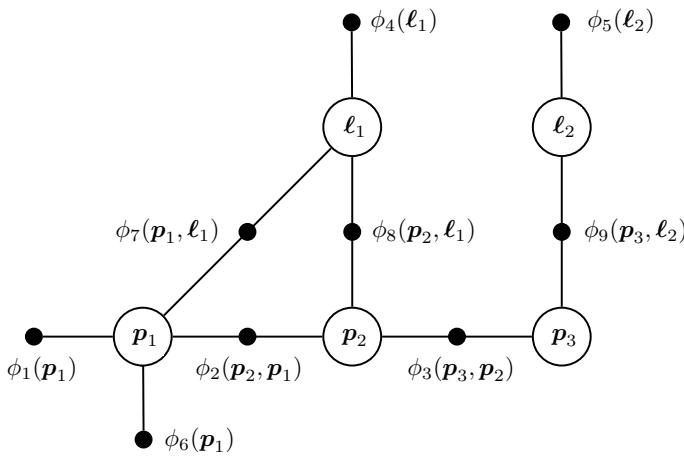
\includegraphics[width=\linewidth]{0d4454ba5350193460ee9f212f491ce8f8f7890456553f8baea8c7f096294afa.jpg}
\caption{图 1.3 图 1.1 示例得到的因子图。}
\label{fig:0d4454ba5350193460ee9f212f491ce8f8f7890456553f8baea8c7f096294afa}
\end{figure}

\begin{equation}
\phi (\boldsymbol {p} _ {1}, \boldsymbol {p} _ {2}, \boldsymbol {p} _ {3}, \ell_ {1}, \ell_ {2}) = \phi_ {1} (\boldsymbol {p} _ {1}) \phi_ {2} (\boldsymbol {p} _ {2}, \boldsymbol {p} _ {1}) \phi_ {3} (\boldsymbol {p} _ {3}, \boldsymbol {p} _ {2})\tag{1.5a}
\end{equation}

\begin{equation}
\times \phi_ {4} (\pmb {\ell} _ {1}) \phi_ {5} (\pmb {\ell} _ {2})\tag{1.5b}
\end{equation}

\begin{equation}
\times \phi_ {6} (\pmb {p} _ {1})\tag{1.5c}
\end{equation}

\begin{equation}
\times \phi_ {7} (\boldsymbol {p} _ {1}, \boldsymbol {\ell} _ {1}) \phi_ {8} (\boldsymbol {p} _ {2}, \boldsymbol {\ell} _ {1}) \phi_ {9} (\boldsymbol {p} _ {3}, \boldsymbol {\ell} _ {2}),\tag{1.5d}
\end{equation}

因子与式（1.4a）—（1.4d）中原始概率密度之间的对应关系应当是显而易见的。

因子值只需与相应概率密度成正比即可：任何与状态变量无关的归一化常数都可以省略，不会造成影响。在本例中，上述因子要么来自先验，例如 $\phi_1(\pmb p_1)\propto p(\pmb p_1)$；要么来自测量，例如 $\phi_9(p_3,\ell_2)\propto p(z_4|p_3,\ell_2)$。虽然测量变量 $z_1\ldots z_4$ 没有在因子图中显式显示，但这些因子都隐式地以它们为条件。有时为了使这一点更加明确，也可以将因子写成（例如）$\phi_9(p_3,\ell_2;z_4)$，甚至写成 $\phi_{z_4}(p_3,\ell_2)$。

\subsection{将因子图作为一种语言}

因子图除了为推断提供形式化基础之外，还能帮助我们可视化多种不同形式的 SLAM 问题、洞察问题结构，并充当一种通用语言，使不同团队的实践者能够在统一的概念下交流。图 1.3 中的每个因子都可以看作一个涉及其所连接变量的方程。通常，方程数量远多于未知量，因此必须量化先验信息和测量中的不确定性。这将导出最小二乘形式，从而适当地融合多个信息源的信息。

\begin{figure}[htbp]
\centering
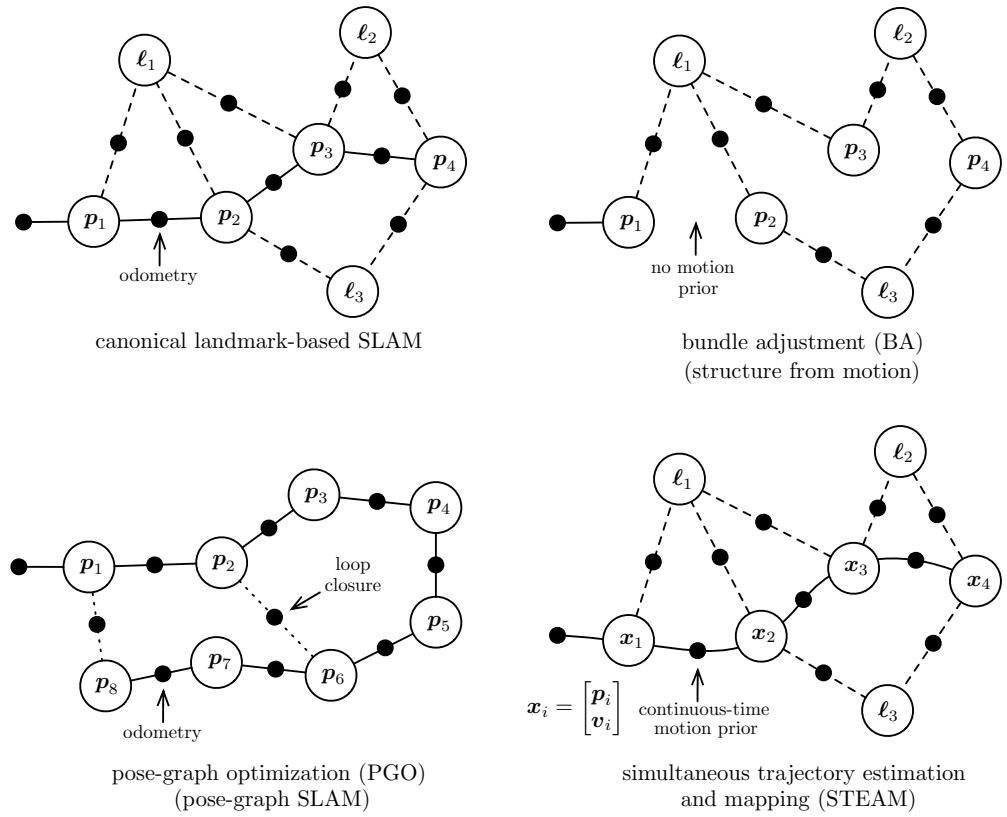
\includegraphics[width=\linewidth]{6a99785c0b3ee0e08985a7267ad8e41222afe130702e8ee950c0d95d9bc80ad6.jpg}
\caption{图 1.4 几种都可以用因子图视角表示的 SLAM 问题变体。典型的基于路标的 SLAM 同时包含位姿变量和路标变量；从位姿观测路标，并且位姿之间通常存在基于里程计的运动先验。束调整（BA）与之相同，但不包含运动先验。位姿图优化（PGO）不含路标变量，但在位姿之间增加了回环测量。最后，同时轨迹估计与建图（STEAM）与基于路标的 SLAM 类似，只是将位姿替换为更高阶状态，并采用平滑的连续时间运动先验。}
\label{fig:6a99785c0b3ee0e08985a7267ad8e41222afe130702e8ee950c0d95d9bc80ad6}
\end{figure}

多种形式的 SLAM 问题都可以很容易地用因子图表示。图 1.1 是基于路标的 SLAM 示例，因为其中同时包含位姿变量和路标变量。图 1.4 给出了其他几种变体，包括束调整（bundle adjustment，BA；与基于路标的 SLAM 相同，但没有运动模型）、位姿图优化（pose-graph optimization，PGO；没有路标变量，但包含位姿之间的回环约束），以及同时轨迹估计与建图（simultaneous trajectory estimation and mapping，STEAM；在位姿中加入速度等导数项）。

\begin{figure}[htbp]
\centering
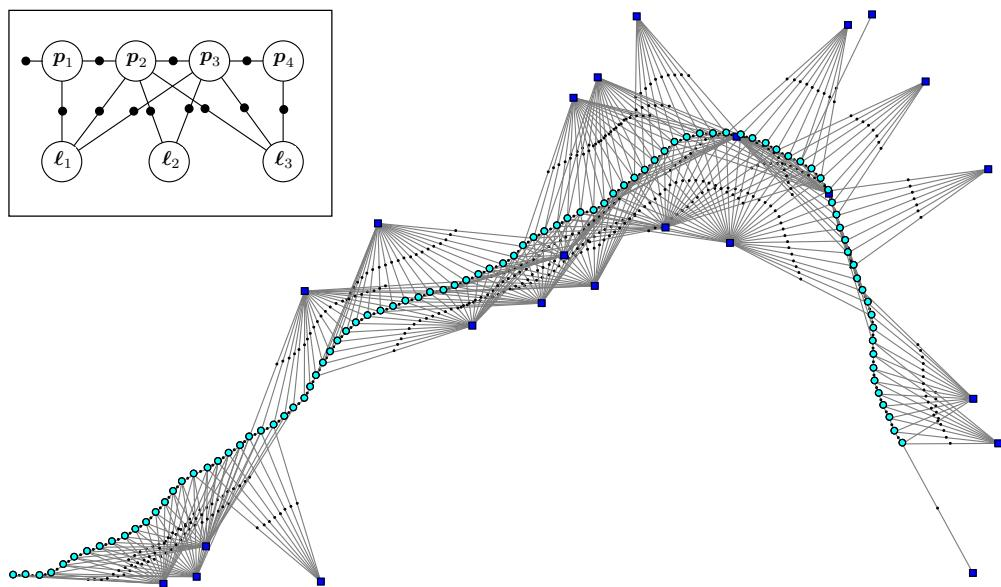
\includegraphics[width=\linewidth]{2d8cd5ffea6b9e14aa6cb1113efedd6424a226fa48a229db8350f93fde3f9e64.jpg}
\caption{图 1.5 一个规模更大的模拟 SLAM 示例因子图。}
\label{fig:2d8cd5ffea6b9e14aa6cb1113efedd6424a226fa48a229db8350f93fde3f9e64}
\end{figure}

比图 1.1 的玩具示例更接近实际的基于路标的 SLAM 问题，其因子图可能类似图 1.5。该图通过模拟一个在平面内运动约 100 个时间步、同时观测路标的二维机器人生成。为便于可视化，每个位姿和路标都按其真实二维位置绘制。可以看到，里程计因子形成了显著的链状骨架，而在两侧则有二元\textsuperscript{2}似然因子连接到约 20 个路标。在这类 SLAM 问题中，除先验之外，所有因子通常都是非线性的。

检查因子图可以揭示大量结构信息，帮助我们理解某个具体的 SLAM 问题实例。首先，有些路标拥有大量测量，我们预计它们会被非常准确地确定；另一些路标与图的联系很弱，因此估计结果也会更不确定。例如，右下方孤立的路标只有一个关联测量。

\section{从 MAP 推断到最小二乘}

最大后验（MAP）推断是确定未知量 $\pmb x$ 取值的过程，使其与不确定测量和先验中包含的信息尽可能一致。在实际情况下，我们并不知道路标的真实位置，也不知道机器人随时间变化的位姿，尽管在许多应用中可能有一个较好的初始估计。下面将说明：在采用高斯测量噪声模型和高斯先验的条件下，MAP 推断对应的优化问题就是我们熟悉的非线性最小二乘问题。

\subsection{用因子图进行 MAP 推断}

给定测量 $\pmb z$，我们关注位姿和/或路标等未知状态变量 $\pmb x$。对于这些未知状态变量，最常用的估计量是最大后验（MAP）估计，其名称源于它最大化了给定测量 $\pmb z$ 时状态 $\pmb x$ 的后验密度 $p(\pmb x|\pmb z)$：

\begin{equation}
\boldsymbol {x} ^ {\mathrm{MAP}} = \underset {\boldsymbol {x}} {\arg \max} p (\boldsymbol {x} | \boldsymbol {z})\tag{1.6a}
\end{equation}

\begin{equation}
= \arg \max _ {\boldsymbol {x}} \frac {p (\boldsymbol {z} | \boldsymbol {x}) p (\boldsymbol {x})}{p (\boldsymbol {z})}\tag{1.6b}
\end{equation}

\begin{equation}
= \underset {\boldsymbol {x}} {\arg \max} p (\boldsymbol {z} | \boldsymbol {x}) p (\boldsymbol {x})\tag{1.6c}
\end{equation}

上式中的第二个等式是贝叶斯定律，它将后验表示为测量密度 $p(\boldsymbol z|\boldsymbol x)$ 与状态先验 $p(\pmb x)$ 的乘积，再用 $p(\boldsymbol z)$ 进行适当归一化。第三个等式省略了 $p(\boldsymbol z)$，因为它与 $\pmb x$ 无关，不会影响求 $\arg\max$ 的结果。换言之，式（1.6c）告诉我们：MAP 估计使似然 $p(\boldsymbol z|\boldsymbol x)$ 与先验 $p(\pmb x)$ 的乘积最大。

我们使用因子图表示未归一化后验 $p(\pmb z|\pmb x)p(\pmb x)$。形式上，因子图 $\boldsymbol F=(\boldsymbol{\mathcal U},\boldsymbol{\mathcal V},\boldsymbol{\mathcal E})$ 是一个二部图，包含两类节点：因子 $\phi_i\in\mathcal U$ 和变量 $\boldsymbol x_j\in\mathcal V$。边 $e_{ij}\in\mathcal E$ 始终连接因子节点和变量节点。与因子 $\phi_i$ 相邻的变量节点集合记作 $\mathcal X(\phi_i)$；我们用 $\boldsymbol\Delta_{\boldsymbol{\mathcal{X}}_i}$ 表示对该集合的一次赋值。按照这些定义，因子图 $F$ 将全局函数 $\phi(\pmb x)$ 定义为

\begin{equation}
\phi (\boldsymbol {x}) = \prod_ {i} \phi_ {i} (\boldsymbol {x} _ {i}).\tag{1.7}
\end{equation}

换言之，独立关系由因子图中的边 $e_{ij}$ 编码；每个因子 $\phi_i$ 只依赖于其邻接集合 $\mathcal X(\phi_i)$ 中的变量 $\boldsymbol\Delta_{\boldsymbol{\mathcal{X}}_i}$。

本章其余部分将说明，如何通过对因子图中的未知变量进行优化，找到最优赋值，即 MAP 估计。对于任意因子图，MAP 推断归结为最大化所有因子图势函数的乘积（式 1.7）：

\begin{equation}
\boldsymbol {x} ^ {\mathrm{MAP}} = \underset {\boldsymbol {x}} {\arg \max} \phi (\boldsymbol {x})\tag{1.8a}
\end{equation}

\begin{equation}
= \underset {\boldsymbol {x}} {\arg \max} \prod_ {i} \phi_ {i} (\boldsymbol {x} _ {i}).\tag{1.8b}
\end{equation}

接下来需要推导因子 $\phi_i(\pmb x_i)$ 的具体形式，而这在很大程度上取决于测量模型 $p(\boldsymbol z|\boldsymbol x)$ 和先验密度 $p(\pmb x)$ 的建模方式。下面将详细讨论。

\subsection{指定概率密度}

上述密度 $p(\boldsymbol z|\boldsymbol x)$ 和 $p(\pmb x)$ 的具体形式高度依赖于应用和所使用的传感器。最常用的密度是多元高斯密度，其概率密度为

\begin{equation}
\mathcal {N} (\boldsymbol {\theta}; \boldsymbol {\mu}, \boldsymbol {\Sigma}) = \frac {1}{\sqrt {| 2 \pi \boldsymbol {\Sigma} |}} \exp \left(- \frac {1}{2} \| \boldsymbol {\theta} - \boldsymbol {\mu} \| _ {\boldsymbol {\Sigma}} ^ {2}\right),\tag{1.9}
\end{equation}

其中，$\pmb\mu\in\mathbb R^n$ 为均值，$\pmb\Sigma$ 为 $n\times n$ 协方差矩阵，并且

\begin{equation}
\| \boldsymbol {\theta} - \boldsymbol {\mu} \| _ {\boldsymbol {\Sigma}} ^ {2} \triangleq (\boldsymbol {\theta} - \boldsymbol {\mu}) ^ {\top} \boldsymbol {\Sigma} ^ {- 1} (\boldsymbol {\theta} - \boldsymbol {\mu})\tag{1.10}
\end{equation}

表示平方马氏距离。归一化常数 $\sqrt{|2\pi\Sigma|}=(2\pi)^{n/2}|\pmb\Sigma|^{1/2}$，其中 $|\cdot|$ 表示矩阵行列式，它保证多元高斯密度在其定义域上的积分为 1。

未知量的先验通常用高斯密度指定；在许多情况下，将测量建模为受到零均值高斯噪声污染既合理又方便。例如，给定位姿 $p$ 到给定路标 $\ell$ 的方位测量\textsuperscript{3} 可建模为

\begin{equation}
\boldsymbol {z} = \boldsymbol {h} (\boldsymbol {p}, \ell) + \boldsymbol {\eta},\tag{1.11}
\end{equation}

其中 $h(\cdot)$ 是测量预测函数，噪声 $\pmb\eta$ 服从协方差为 $\Sigma_R$ 的零均值高斯密度。于是，关于测量 $\boldsymbol z$ 的条件密度 $p(\boldsymbol z|\boldsymbol p,\boldsymbol\ell)$ 为

\begin{equation}
p (\boldsymbol {z} | \boldsymbol {p}, \ell) = \mathcal {N} (\boldsymbol {z}; \boldsymbol {h} (\boldsymbol {p}, \ell), \boldsymbol {\Sigma} _ {\boldsymbol {R}}) = \frac {1}{\sqrt {| 2 \pi \boldsymbol {\Sigma} _ {\boldsymbol {R}} |}} \exp \left(- \frac {1}{2} \| \boldsymbol {z} - \boldsymbol {h} (\boldsymbol {p}, \ell) \| _ {\boldsymbol {\Sigma} _ {\boldsymbol {R}}} ^ {2}\right).\tag{1.12}
\end{equation}

在实际机器人应用中，测量函数 $h(\cdot)$ 往往是非线性的。不过，尽管它取决于所使用的传感器和 SLAM 前端，但通常并不难理解或写出。二维方位测量的测量函数就是

\begin{equation}
\pmb {h} (\pmb {p}, \ell) = \mathrm{atan2} (\ell_ {y} - p _ {y}, \ell_ {x} - p _ {x}),\tag{1.13}
\end{equation}

其中 $\ell_x,\ell_y$ 是路标的 $x,y$ 坐标，$p_x,p_y$ 是位姿的 $x,y$ 坐标，atan2 是众所周知的双参数反正切函数。因此，最终的概率测量模型 $p(\boldsymbol z|\boldsymbol p,\boldsymbol\ell)$ 为

\begin{equation}
p (\pmb {z} | \pmb {p}, \pmb {\ell}) = \frac {1}{\sqrt {| 2 \pi \pmb {\Sigma} _ {\pmb {R}} |}} \exp \left(- \frac {1}{2} \| \pmb {z} - \mathrm{atan2} (\ell_ {y} - p _ {y}, \ell_ {x} - p _ {x}) \| _ {\pmb {\Sigma} _ {\pmb {R}}} ^ {2}\right).\tag{1.14}
\end{equation}

需要注意的是，我们并不总是假设测量噪声为高斯噪声。例如，为了应对偶发的数据关联错误，许多作者提出使用具有更重尾部的鲁棒测量密度；第 3 章将讨论这些方法。

并非所有涉及的概率密度都来自测量。例如，在玩具 SLAM 问题中，轨迹先验 $p(\pmb x)$ 由先验 $p(\pmb p_1)$ 和条件密度 $p(\pmb p_{t+1}|\pmb p_t)$ 构成，用于描述在给定已知控制输入 $\pmb u_t$ 的条件下机器人所遵循的概率运动模型。实践中，我们通常采用条件高斯假设：

\begin{equation}
p (\pmb {p} _ {t + 1} | \pmb {p} _ {t}, \pmb {u} _ {t}) = \frac {1}{\sqrt {| 2 \pi \pmb {\Sigma} _ {Q} |}} \exp \left(- \frac {1}{2} \| \pmb {p} _ {t + 1} - \pmb {g} (\pmb {p} _ {t}, \pmb {u} _ {t}) \| _ {\pmb {\Sigma} _ {Q}} ^ {2}\right),\tag{1.15}
\end{equation}

其中 $g(\cdot)$ 是运动模型，$\Sigma_Q$ 是维度适当的协方差矩阵；例如，对于在平面内运动的机器人，它是 $3\times3$ 矩阵。

我们经常没有已知的控制输入 $\pmb u_t$，而是测量机器人如何运动，例如通过里程计测量 $\pmb o_t$。若假设里程计只是测量位姿差，并受到协方差为 $\Sigma_S$ 的高斯噪声影响，则有

\begin{equation}
p (\boldsymbol {o} _ {t} | \boldsymbol {p} _ {t + 1}, \boldsymbol {p} _ {t}) = \frac {1}{\sqrt {| 2 \pi \boldsymbol {\Sigma} _ {S} |}} \exp \left(- \frac {1}{2} \| \boldsymbol {o} _ {t} - (\boldsymbol {p} _ {t + 1} - \boldsymbol {p} _ {t}) \| _ {\boldsymbol {\Sigma} _ {S}} ^ {2}\right).\tag{1.16}
\end{equation}

如果同时拥有已知控制输入 $\pmb u_t$ 和里程计测量 $\pmb o_t$，就可以将式（1.15）与式（1.16）结合起来。

对于在三维空间中运行的机器人，需要使用稍微复杂一些的工具，为 SE(3) 这类非线性流形指定概率密度；下一章将对此进行讨论。

\subsection{非线性最小二乘}

现在说明，对于采用上述高斯噪声模型的 SLAM 问题，MAP 推断等价于求解非线性最小二乘问题。假设所有因子都与多元高斯分布成正比，即

\begin{equation}
\phi_ {i} (\boldsymbol {x} _ {i}) \propto \exp \left(- \frac {1}{2} \| \boldsymbol {z} _ {i} - \boldsymbol {h} _ {i} (\boldsymbol {x} _ {i}) \| _ {\boldsymbol {\Sigma} _ {i}} ^ {2}\right).\tag{1.17}
\end{equation}

这既包括简单的高斯先验因子，也包括由零均值正态分布噪声污染的测量所导出的似然因子。将式（1.17）代入式（1.8b），取负对数并去掉因子 $1/2$，便可转而最小化一组非线性最小二乘项之和：

\begin{equation}
\boldsymbol {x} ^ {\mathrm{MAP}} = \underset {\boldsymbol {x}} {\arg \min} \sum_ {i} \| \boldsymbol {z} _ {i} - \boldsymbol {h} _ {i} (\boldsymbol {x} _ {i}) \| _ {\boldsymbol {\Sigma} _ {i}} ^ {2}.\tag{1.18}
\end{equation}

最小化这个目标函数，就是将多个由测量得到的因子以及可能存在的多个先验结合起来，执行传感器融合，从而确定未知量的 MAP 解。

一个重要而不太显然的观察是，式（1.18）中的因子通常只描述所涉及未知变量 $\boldsymbol\Delta_{\boldsymbol{\mathcal{X}}_i}$ 的部分概率。除简单的先验因子外，测量 $z_i$ 的维度通常低于未知量 $\boldsymbol\Delta_{\boldsymbol{\mathcal{X}}_i}$ 的维度。在这种情况下，单个因子会为 $\pmb x_i$ 定义域中的一个无限子集赋予相同的似然。例如，相机图像中的一个二维测量，与一整条能够投影到该图像位置的三维点射线相容。

尽管函数 $\pmb h_i$ 是非线性的，但如果有一个足够好的初始猜测，本章讨论的非线性优化方法通常能够收敛到式（1.18）的全局最小值。不过需要提醒的是，式（1.18）的目标函数是非凸的，因此当初始猜测较差时，无法保证不会陷入局部最小值。这促成了所谓的\textbf{可证明最优求解器}，第 6 章将对此进行介绍。下面我们先关注局部方法，而不是全局求解器；首先考虑更容易的线性化问题。

\section{求解线性最小二乘}

在处理更困难的非线性最小二乘之前，本节首先说明如何将问题线性化，展示线性化如何导出线性最小二乘问题，并回顾如何通过矩阵分解高效求解相应的正规方程。关于这些方法的经典参考是 Golub 和 Van Loan 的著作 \textsuperscript{[389]}。

\subsection{线性化}

可以使用简单的泰勒展开，将非线性最小二乘目标函数（式 1.18）中的所有测量函数 $\pmb h_i(\cdot)$ 线性化：

\begin{equation}
\boldsymbol {h} _ {i} (\boldsymbol {x} _ {i}) = \boldsymbol {h} _ {i} (\boldsymbol {x} _ {i} ^ {0} + \boldsymbol {\delta} _ {i}) \approx \boldsymbol {h} _ {i} (\boldsymbol {x} _ {i} ^ {0}) + \boldsymbol {H} _ {i} \boldsymbol {\delta} _ {i},\tag{1.19}
\end{equation}

其中，测量雅可比 $\pmb H_i$ 定义为在给定线性化点 $\pmb x_i^0$ 处 $\pmb h_i(\cdot)$ 的（多元）偏导数：

\begin{equation}
\boldsymbol {H} _ {i} \triangleq \left. \frac {\partial \boldsymbol {h} _ {i} (\boldsymbol {x} _ {i})}{\partial \boldsymbol {x} _ {i}} \right| _ {\boldsymbol {x} _ {i} ^ {0}},\tag{1.20}
\end{equation}

而 $\pmb\delta_i\triangleq\pmb x_i-\pmb x_i^0$ 是状态更新向量。这里假设 $\boldsymbol\Delta_{\boldsymbol{\mathcal{X}}_i}$ 位于向量空间中，或者等价地，可以用向量表示。当 $\pmb x$ 中的一些未知状态表示三维旋转或其他更复杂的流形类型时，情况并不总是如此。第 2 章将重新讨论这个问题。

将泰勒展开（式 1.19）代入非线性最小二乘表达式（式 1.18），得到关于状态更新向量 $\pmb\delta$ 的线性最小二乘问题：

\begin{equation}
\boldsymbol {\delta} ^ {*} = \underset {\boldsymbol {\delta}} {\arg \min} \sum_ {i} \left\| \boldsymbol {z} _ {i} - \boldsymbol {h} _ {i} (\boldsymbol {x} _ {i} ^ {0}) - \boldsymbol {H} _ {i} \boldsymbol {\delta} _ {i} \right\| _ {\boldsymbol {\Sigma} _ {i}} ^ {2}\tag{1.21a}
\end{equation}

\begin{equation}
= \arg \min _ {\boldsymbol {\delta}} \sum_ {i} \left\| \left(\boldsymbol {z} _ {i} - \boldsymbol {h} _ {i} (\boldsymbol {x} _ {i} ^ {0})\right) - \boldsymbol {H} _ {i} \boldsymbol {\delta} _ {i} \right\| _ {\boldsymbol {\Sigma} _ {i}} ^ {2},\tag{1.21b}
\end{equation}

其中，$z_i-h_i(x_i^0)$ 是线性化点处的预测误差，即实际测量与预测测量之间的差。上式中的 $\pmb\delta^*$ 表示局部线性化问题的解。

通过一个简单的变量替换，从这里开始可以去掉协方差矩阵 $\Sigma_i$：将 $\pmb\Sigma^{1/2}$ 定义为 $\Sigma$ 的矩阵平方根，则平方马氏范数可以改写为：

其中

\begin{equation}
\left\| \boldsymbol {e} \right\| _ {\boldsymbol {\Sigma}} ^ {2} \stackrel {{\Delta}} {{=}} \boldsymbol {e} ^ {\top} \boldsymbol {\Sigma} ^ {- 1} \boldsymbol {e} = \left(\boldsymbol {\Sigma} ^ {- 1 / 2} \boldsymbol {e}\right) ^ {\top} \left(\boldsymbol {\Sigma} ^ {- 1 / 2} \boldsymbol {e}\right) = \left\| \boldsymbol {\Sigma} ^ {- 1 / 2} \boldsymbol {e} \right\| _ {2} ^ {2}.\tag{1.22}
\end{equation}

因此，只需在式（1.21b）的每一项中，用 $\pmb\Sigma_i^{-1/2}$ 左乘雅可比和预测误差，就可以消除协方差矩阵 $\Sigma_i$：

\begin{equation}
\pmb {A} _ {i} = \pmb {\Sigma} _ {i} ^ {- 1 / 2} \pmb {H} _ {i}\tag{1.23a}
\end{equation}

\begin{equation}
\pmb {b} _ {i} = \pmb {\Sigma} _ {i} ^ {- 1 / 2} \left(\pmb {z} _ {i} - \pmb {h} _ {i} (\pmb {x} _ {i} ^ {0})\right).\tag{1.23b}
\end{equation}

这个过程称为\textbf{白化}。例如，对于标量测量，它仅仅意味着将每一项除以测量标准差 $\sigma_i$。注意，这一步消除了测量的单位（例如长度、角度），因此不同的行可以组合到同一个代价函数中。

\subsection{将 SLAM 写成线性最小二乘}

线性化后，最终得到如下标准最小二乘问题：

\begin{equation}
\boldsymbol {\delta} ^ {*} = \underset {\boldsymbol {\delta}} {\arg \min} \sum_ {i} \| \boldsymbol {A} _ {i} \boldsymbol {\delta} _ {i} - \boldsymbol {b} _ {i} \| _ {2} ^ {2}\tag{1.24a}
\end{equation}

\begin{equation}
= \underset {\boldsymbol {\delta}} {\arg \min} \| \boldsymbol {A} \boldsymbol {\delta} - \boldsymbol {b} \| _ {2} ^ {2}.\tag{1.24b}
\end{equation}

这里的 $A$ 和 $b$ 分别由收集所有白化雅可比矩阵 $\pmb A_i$ 以及白化预测误差 $\pmb b_i$ 得到，并将它们组合成一个大的矩阵 $A$ 和右端项向量 $b$。

雅可比矩阵 $A$ 是一个规模很大但稀疏的矩阵，其分块结构与底层因子图的结构相对应。下面将详细考察这种稀疏结构。不过首先回顾经典线性代数方法，说明如何求解这个最小二乘问题。

\subsection{用矩阵分解求解最小二乘}

对于一个满列秩的 $m\times n$ 矩阵 $A$（$m\ge n$），式（1.24b）的唯一最小二乘解可以通过求解正规方程获得：

\begin{equation}
\left(\boldsymbol {A} ^ {\top} \boldsymbol {A}\right) \boldsymbol {\delta} ^ {*} = \boldsymbol {A} ^ {\top} \boldsymbol {b}.\tag{1.25}
\end{equation}

通常的做法是分解信息矩阵（也称 Hessian 矩阵）$\pmb\Lambda$：

\begin{equation}
\boldsymbol {\Lambda} \stackrel {\Delta} {=} \boldsymbol {A} ^ {\top} \boldsymbol {A} = \boldsymbol {R} ^ {\top} \boldsymbol {R}.\tag{1.26}
\end{equation}

这里的 Cholesky 因子 $R$ 是一个 $n\times n$ 的上三角矩阵\textsuperscript{4}，通过 Cholesky 分解计算得到；Cholesky 分解是针对对称正定矩阵的 LU（下三角—上三角）分解变体。随后，先求解

\begin{equation}
\boldsymbol {R} ^ {\top} \boldsymbol {y} = \boldsymbol {A} ^ {\top} \boldsymbol {b}\tag{1.27}
\end{equation}

得到 $y$，再通过前代和回代求解

\begin{equation}
\boldsymbol {R} \delta^ {*} = \boldsymbol {y}\tag{1.28}
\end{equation}

得到 $\delta^*$。对于稠密矩阵，Cholesky 分解需要 $n^3/3$ 次浮点运算；整个算法（包括计算对称矩阵 $A^\top A$ 的一半）需要 $(m+n/3)n^2$ 次浮点运算。还可以使用 LDL\textsuperscript{\textbackslash\{\}top} 分解，这是 Cholesky 分解的一个变体，可以避免开平方根。

另一种比 Cholesky 分解更准确、数值稳定性更好的方法是 QR 分解。该方法不必显式计算信息矩阵 $\pmb\Lambda$，而是直接对 $A$ 及其右端项进行 QR 分解：

\begin{equation}
\boldsymbol {A} = \boldsymbol {Q} \left[ \begin{array}{c} \boldsymbol {R} \\ \boldsymbol {0} \end{array} \right], \quad \left[ \begin{array}{c} \boldsymbol {d} \\ \boldsymbol {e} \end{array} \right] = \boldsymbol {Q} ^ {\top} \boldsymbol {b}.\tag{1.29}
\end{equation}

其中，$Q$ 是 $m\times m$ 正交矩阵，$d\in\mathbb R^n$，$e\in\mathbb R^{m-n}$，而 $R$ 是同一个上三角 Cholesky 三角因子。对于稠密矩阵 $A$，通常按列从左到右计算 $R$。对每一列 $j$，通过用 Householder 反射矩阵 $H_j$ 左乘 $A$，将对角线下方的所有非零元素置零。经过 $n$ 次迭代，$A$ 完全分解为

\begin{equation}
\boldsymbol {H} _ {n} \dots \boldsymbol {H} _ {2} \boldsymbol {H} _ {1} \boldsymbol {A} = \boldsymbol {Q} ^ {\top} \boldsymbol {A} = \left[ \begin{array}{c} \boldsymbol {R} \\ \boldsymbol {0} \end{array} \right].\tag{1.30}
\end{equation}

通常不会显式构造正交矩阵 $Q$，而是将 $b$ 作为额外一列附加到 $A$，直接计算变换后的右端项 $Q^\top b$。由于 $Q$ 是正交矩阵，有

\begin{equation}
\left\| \boldsymbol {A} \delta - \boldsymbol {b} \right\| _ {2} ^ {2} = \left\| \boldsymbol {Q} ^ {\top} \boldsymbol {A} \delta - \boldsymbol {Q} ^ {\top} \boldsymbol {b} \right\| _ {2} ^ {2} = \left\| \boldsymbol {R} \delta - \boldsymbol {d} \right\| _ {2} ^ {2} + \left\| \boldsymbol {e} \right\| _ {2} ^ {2}.\tag{1.31}
\end{equation}

其中使用了式（1.29）的等式。显然，$\|e\|_2^2$ 就是最小二乘残差平方和，而最小二乘解 $\delta^*$ 可以通过回代求解三角系统

\begin{equation}
\boldsymbol {R} \delta^ {*} = \boldsymbol {d}\tag{1.32}
\end{equation}

得到。注意，QR 分解得到的上三角因子 $R$（对角线上的符号可能不同）与 Cholesky 分解得到的因子相同，因为

\begin{equation}
\boldsymbol {A} ^ {\top} \boldsymbol {A} = \left[ \begin{array}{c} \boldsymbol {R} \\ \boldsymbol {0} \end{array} \right] ^ {\top} \boldsymbol {Q} ^ {\top} \boldsymbol {Q} \left[ \begin{array}{c} \boldsymbol {R} \\ \boldsymbol {0} \end{array} \right] = \boldsymbol {R} ^ {\top} \boldsymbol {R}.\tag{1.33}
\end{equation}

这里再次使用了 $Q$ 为正交矩阵这一事实。QR 的计算成本主要来自 Householder 反射，为 $2(m-n/3)n^2$ 次浮点运算。与 Cholesky 相比，当 $m\gg n$ 时，两种算法都需要 $O(mn^2)$ 次运算，但 QR 分解大约慢两倍。

总之，与 SLAM 线性化优化问题相关的线性代数可以简洁地概括为：将信息矩阵 $\pmb\Lambda$ 或测量雅可比矩阵 $A$ 分解成平方根形式。由于它们都基于 SAM 问题中的矩阵平方根，我们将这类方法称为平方根 SAM，简称 SAM \textsuperscript{[249, 254]}。

\section{非线性优化}

本节讨论求解式（1.18）所定义非线性最小二乘问题的一些经典优化方法。回顾一下，SLAM 中的非线性最小二乘目标函数为

\begin{equation}
J (\boldsymbol {x}) \triangleq \sum_ {i} \| \boldsymbol {z} _ {i} - \boldsymbol {h} _ {i} (\boldsymbol {x} _ {i}) \| _ {\boldsymbol {\Sigma} _ {i}} ^ {2}.\tag{1.34}
\end{equation}

它对应于一个由测量以及部分或全部未知量的先验密度共同构成的非线性因子图。

一般来说，非线性最小二乘问题无法直接求解，而需要从合适的初始估计出发迭代求解。非线性优化方法通过依次求解式（1.18）的线性近似，逐渐逼近最小值 \textsuperscript{[264]}。不同算法在局部近似代价函数的方式，以及根据这种局部近似寻找改进估计的方式上有所不同。关于非线性求解器的深入综述见 \textsuperscript{[814]}；\textsuperscript{[389]} 则从线性代数角度进行讨论。

所有算法都具有如下基本结构：从初始估计 $\pmb x^0$ 出发，在每次迭代中计算更新步 $\pmb\delta$，并将其应用到下一次估计 $\pmb x^{t+1}=\pmb x^t+\pmb\delta$。当达到某些收敛准则时停止，例如变化量 $\pmb\delta$ 的范数低于一个很小的阈值。

\subsection{最速下降}

最速下降（steepest descent，SD）使用当前估计处的最速下降方向来计算更新步：

\begin{equation}
\pmb {\delta} ^ {\mathrm{sd}} = - \alpha \left. \nabla J (\pmb {x}) \right| _ {\pmb {x} = \pmb {x} ^ {t}},\tag{1.35}
\end{equation}

其中 $\pmb x^t$ 是当前的 $x$ 估计。这里使用负梯度确定最速下降方向。对于非线性最小二乘目标函数（式 1.34），在当前点附近将目标函数近似为二次函数 $J(\pmb x)\approx\|\pmb A(\pmb x-\pmb x^t)-\pmb b\|_2^2$，在该线性化点可以得到精确梯度

\begin{equation*}
\left.\nabla J(\pmb x)\right|_{\pmb x=\pmb x^t}=-2\pmb A^\top\pmb b.
\end{equation*}

步长 $\alpha$ 必须谨慎选择，以平衡更新的安全性与合理的收敛速度。可以执行显式线搜索，在给定方向上寻找最小值。SD 算法简单，但在最小值附近收敛较慢。

\subsection{高斯—牛顿}

高斯—牛顿（Gauss—Newton，GN）通过使用二阶更新实现更快收敛。GN 利用非线性最小二乘问题的特殊结构，用 $A^\top A$ 近似 Hessian 矩阵。GN 更新步通过求解正规方程（式 1.25）得到：

\begin{equation}
\boldsymbol {A} ^ {\top} \boldsymbol {A} \delta^ {\mathrm{gn}} = \boldsymbol {A} ^ {\top} \boldsymbol {b}.\tag{1.36}
\end{equation}

可以使用第 1.3.3 节中的任意方法求解。对于行为良好（即近似二次）的目标函数和较好的初始估计，高斯—牛顿表现出近似二次的收敛速度。如果二次近似很差，GN 步可能使新估计远离最小值，随后发生发散。

\subsection{Levenberg—Marquardt}

Levenberg—Marquardt（LM）算法允许多次迭代直至收敛，同时控制我们愿意信任高斯—牛顿二次近似的区域。因此，这类方法通常称为\textbf{信赖域方法}。

为了结合 SD 和 GN 的优点，Levenberg \textsuperscript{[646]} 提议在正规方程（式 1.25）的对角线上加入非负常数 $\lambda\in\mathbb R^+\cup\{0\}$：

\begin{equation}
\left(\boldsymbol {A} ^ {\top} \boldsymbol {A} + \lambda \mathbf {I}\right) \boldsymbol {\delta} ^ {\mathrm{lm}} = \boldsymbol {A} ^ {\top} \boldsymbol {b}.\tag{1.37}
\end{equation}

当 $\lambda=0$ 时得到 GN；当 $\lambda$ 很大时，近似有 $\delta^*\approx\frac1\lambda A^\top b$，即沿代价函数 $J$（式 1.34）的负梯度方向更新。因此，LM 可以看作在 GN 和 SD 之间自然地进行折中。

随后 Marquardt \textsuperscript{[731]} 提议考虑对角元素的尺度，以获得更快的收敛：

\begin{equation}
\left(\boldsymbol {A} ^ {\top} \boldsymbol {A} + \lambda \operatorname{diag} (\boldsymbol {A} ^ {\top} \boldsymbol {A})\right) \boldsymbol {\delta} ^ {\mathrm{lm}} = \boldsymbol {A} ^ {\top} \boldsymbol {b}.\tag{1.38}
\end{equation}

这一修改会在梯度较小（目标函数近似平坦的方向）时沿最速下降方向采取更大的步长，因为此时对角元素的逆会较大；相反，在目标函数变化陡峭的方向上，算法会更加谨慎并采取更小的步长。对正规方程的这两种修改，都可以从贝叶斯角度解释为：给问题中的所有未知变量加入零均值先验。

GN 与 LM 的一个关键区别是，LM 会拒绝使残差平方和增大的更新。被拒绝意味着非线性函数在局部表现不佳，需要采取更小的步长。实现方式是启发式地增大 $\lambda$，例如将当前值乘以 10，然后重新求解修改后的正规方程。另一方面，如果某一步使残差平方和降低，则接受该更新，并相应地更新状态估计；此时减小 $\lambda$（例如除以 10），然后以新的线性化点重复算法，直至收敛。

\subsection{Dogleg 最小化}

Powell 的 dogleg（PDL）算法 \textsuperscript{[885]} 可以作为 LM 的更高效替代方案 \textsuperscript{[697]}。Levenberg—Marquardt 算法的一个主要缺点是：如果某一步被拒绝，就必须重新分解修改后的信息矩阵，而这正是算法中最昂贵的环节。因此，PDL 的核心思想是分别计算 GN 步和 SD 步，再将二者适当地组合起来。如果 LM 步被拒绝，GN 步和 SD 步的方向仍然有效，可以用另一种方式组合，直到代价下降。因此，状态估计的每次更新只需进行一次矩阵分解，而不是多次。

图 1.6 展示了 GN 步和 SD 步的组合方式。组合步从 SD 更新开始，随后急转弯（因此称为 dogleg，即“狗腿”）朝向 GN 更新，但在信赖域边界处停止。与 LM 不同，PDL 显式维护一个信赖域，在该区域内我们相信线性假设。线性近似是否合适由增益比决定：

\begin{equation}
\rho = \frac {J (\boldsymbol {x} ^ {t}) - J (\boldsymbol {x} ^ {t} + \boldsymbol {\delta})}{L (\boldsymbol {0}) - L (\boldsymbol {\delta})},\tag{1.39}
\end{equation}

其中 $L(\delta)=\pmb A^\top\pmb A\delta-\pmb A^\top\pmb b$ 是在当前估计 $\pmb x^t$ 处对式（1.34）非线性二次代价函数 $J$ 的线性化。如果 $\rho$ 很小（即 $\rho<0.25$），说明代价下降幅度没有达到线性化预测，因而缩小信赖域。相反，如果实际下降与预测相符或更好（即 $\rho>0.75$），则根据更新向量的大小扩大信赖域，并接受该步。

\section{因子图与稀疏性}

到目前为止介绍的求解器假设相关矩阵可以是稠密的；但在 SLAM 中，稠密方法无法扩展到实际问题规模。对于图 1.1 的玩具问题，稠密方法能够正常工作。图 1.5 所示的较大模拟问题更接近真实世界，不过对于 SLAM 而言它仍然相对较小，因为实际问题常常包含数千乃至数百万个未知量。我们之所以仍能处理这类问题，正是因为其稀疏性。

直接观察因子图即可认识到这种稀疏性。由图 1.5 可见，该图是稀疏的（远非完全连接图）。连接 100 个未知位姿的里程计链，是由 100 个二元因子构成的线性结构，而不是可能存在的 $100^2$ 个（二元）因子。此外，对于 20 个路标，最多可以有 2000 个因子将每个路标与每个位姿相连，但实际数量更接近 400。最后，路标之间完全没有因子，这反映了我们没有获得它们相对位置的任何信息。这种结构是大多数 SLAM 问题的典型特征。

\subsection{稀疏雅可比矩阵及其因子图}

现代 SLAM 算法的关键在于利用稀疏性。SLAM 中因子图的一个重要性质是：它准确表示了最终稀疏雅可比矩阵 $A$ 的稀疏分块结构。为此，重新考察非线性 SLAM 问题内循环中的关键计算——最小二乘问题：

\begin{equation}
\boldsymbol {\delta} ^ {*} = \underset {\boldsymbol {\delta}} {\arg \min} \sum_ {i} \| \boldsymbol {A} _ {i} \boldsymbol {\delta} _ {i} - \boldsymbol {b} _ {i} \| _ {2} ^ {2}.\tag{1.40}
\end{equation}

上式每一项都来自原始非线性 SLAM 问题中的一个因子，并在当前线性化点附近进行线性化（式 1.21b）。矩阵 $A_i$ 可以按变量拆分成若干分块，并收集成一个大的分块稀疏雅可比矩阵，其稀疏结构恰好由因子图给出。

尽管这些线性问题通常作为非线性优化的内部迭代出现，下面省略更新量的上标，因为相关结论对其来源无关，适用于一般线性问题。

考虑图 1.1 玩具示例的因子图。线性化后得到具有图 1.7 所示分块结构的稀疏系统 $[A\ b]$。将其与因子图进行比较可以发现：每个因子对应一个分块行，每个变量对应 $A$ 的一个分块列。总共有 9 个分块行，分别对应因子分解 $\phi(p_1,p_2,p_3,\ell_1,\ell_2)$ 中的 9 个因子。

\begin{figure}[htbp]
\centering
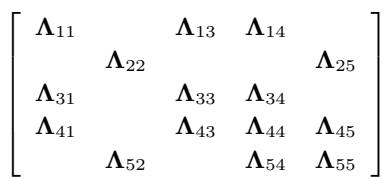
\includegraphics[width=\linewidth]{9e5631051f6c2aeb5026d609b884773bd2902fc60e87816bfa9f5ecda4ab10d4.jpg}
\caption{图 1.7 图 1.1 玩具 SLAM 示例的稀疏雅可比矩阵 $A$ 的分块结构，其中空白项为零。}
\label{fig:9e5631051f6c2aeb5026d609b884773bd2902fc60e87816bfa9f5ecda4ab10d4}
\end{figure}

\subsection{稀疏信息矩阵及其图}

如第 1.3.3 节所述，使用 Cholesky 分解求解正规方程时，首先要形成 Hessian 矩阵或信息矩阵 $\pmb\Lambda=A^\top A$。注意，$A^\top A$ 并不是真正的 Hessian，而是由残差的泰勒级数截断得到的“高斯—牛顿”近似。一般而言，由于雅可比 $A$ 是分块稀疏的，Hessian $\pmb\Lambda$ 也应当是稀疏的。按构造，$\pmb\Lambda$ 是对称矩阵；当唯一 MAP 解存在时，它还是正定的。

信息矩阵 $\pmb\Lambda$ 的稀疏模式自然定义了一个无向图 $G$：如果两个变量曾经共同出现在同一个因子中，它们之间就存在一条边。在分块层面，$\pmb\Lambda=A^\top A$ 的稀疏模式正好是该图的邻接矩阵。这一结论不限于二元因子：一个 n 元因子会在其全部变量之间诱导一个团，因此对应所有变量对之间的非零分块。

图 1.8 展示了（a）玩具示例信息矩阵 $\pmb\Lambda$ 的分块结构，以及（b）对应的无向图 $G$。下面经常使用与 $\pmb\Lambda$ 关联的图 $G$ 来讨论稀疏性和填充。

\begin{figure}[htbp]
\centering
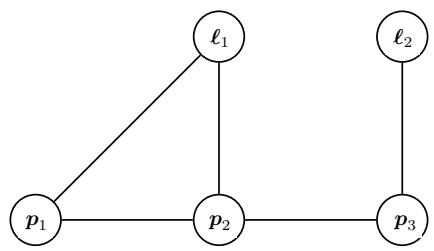
\includegraphics[width=\linewidth]{4f020457cc25171d369116da03c553cf2f3bd9c2efab51f4b769b89ac0e14913.jpg}
\caption{图 1.8 玩具 SLAM 问题的信息矩阵 $\pmb\Lambda$ 及其关联的无向图 $G$。}
\label{fig:4f020457cc25171d369116da03c553cf2f3bd9c2efab51f4b769b89ac0e14913}
\end{figure}

\subsection{稀疏分解}

我们已经看到，MAP 估计等价于求解第 1.3.3 节所述的线性方程组；对于非线性最小二乘问题，则在迭代过程中反复求解这类系统。前两节说明，$A$ 和 $A^\top A$ 都具有由因子图决定的稀疏性。无需展开细节，这种已知的稀疏模式可以显著加速 Cholesky 分解（处理 $A^\top A$ 时）或 QR 分解（处理 $A$ 时）。例如，CHOLMOD \textsuperscript{[189]} 和 SuiteSparseQR \textsuperscript{[240]} 都提供了高效实现，许多软件包在底层使用它们。实践中，在稀疏问题上，稀疏 Cholesky 或 LDU 分解通常也优于 QR 分解，而且优势并非只是一个常数因子。

稀疏分解所需的浮点运算量远低于稠密矩阵。关键在于，稀疏矩阵采用的列排序会显著影响总计算量。任何排序最终都会产生相同的 MAP 估计，但变量排序决定矩阵因子中的填充量（即超出待分解矩阵原有稀疏模式的额外非零项）。已知寻找使矩阵分解填充最小的变量排序是 NP-hard 问题 \textsuperscript{[1239]}，因此必须采用良好的启发式方法，这将进一步影响分解算法的计算复杂度。

仍以图 1.5 所示的较大模拟示例说明这一点。图 1.9 展示了对应稀疏雅可比矩阵 $A$ 的模式，并在右上角给出信息矩阵 $\pmb\Lambda=A^\top A$ 的模式。图右侧还给出了两种不同排序下得到的上三角 Cholesky 因子 $R$。两者都具有稀疏性，也都满足 $R^\top R=A^\top A$（变量置换除外），但稀疏程度不同，而这正决定了分解 $A$ 的代价。第一种排序最自然：先排列位姿，再排列路标，得到的稀疏 $R$ 因子有 9399 个非零项。相比之下，右下角按列近似最小度（COLAMD）启发式方法 \textsuperscript{[29, 241]} 重新排序后得到的 $R$ 因子只有 4168 个非零项。然而，回代会为两种排序给出完全相同的解。

还可以使用预条件共轭梯度等工具迭代求解正规方程。在具有特殊稀疏模式的视觉 SLAM 中，幂迭代也已取得成功 \textsuperscript{[1171]}。不过，对于大多数 SLAM 问题，稀疏分解仍然是首选方法，而且它还具有很好的图模型解释，下面将对此进行讨论。

\begin{figure}[htbp]
\centering
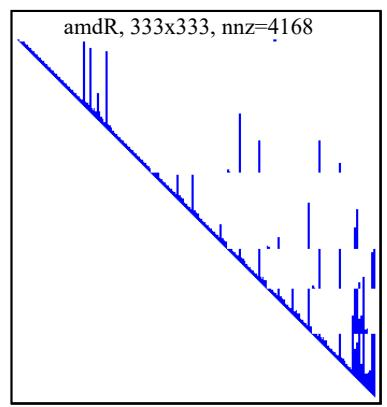
\includegraphics[width=\linewidth]{f5fad5e1ec472a6b428b7a6fe55523c80ff02dd7cd4a0aea9f1935d0fb1fde57.jpg}
\caption{图 1.9 左侧是图 1.5 问题对应的测量雅可比矩阵 $A$；右侧从上到下依次为信息矩阵 $\pmb\Lambda=A^\top A$、其上三角 Cholesky 因子 $R$，以及采用更优变量排序（COLAMD）得到的替代因子 $R$。}
\label{fig:f5fad5e1ec472a6b428b7a6fe55523c80ff02dd7cd4a0aea9f1935d0fb1fde57}
\end{figure}

\section{消元}

到目前为止，我们一直从线性代数角度解释 SLAM 推断。本节将视角扩展到更抽象的层次，直接利用图模型思考推断问题。这最终会引出当前最先进的 SLAM 求解器：下一节中用于增量平滑与建图的贝叶斯树。

\subsection{变量消元算法}

存在一种通用算法，可以针对任意（最好是稀疏的）因子图，计算未知变量 $\pmb x$ 上相应的后验密度 $p(\pmb x|z)$，并将其表示为易于恢复 MAP 解的形式。如前所述，因子图以因子乘积的形式表示未归一化后验 $\phi(\pmb x)\propto p(\pmb x|\pmb z)$；在 SLAM 问题中，该图通常直接由测量生成。变量消元算法提供了一套规则，可将因子图转换为另一个称为\textbf{贝叶斯网络}的图模型，该模型只依赖未知变量 $\pmb x$，从而可以方便地进行 MAP 推断（以及采样、边缘化等其他操作）。

具体来说，变量消元算法可以将如下形式的任意因子图

\begin{equation}
\phi (\boldsymbol {x}) = \phi (\boldsymbol {x} _ {1}, \dots , \boldsymbol {x} _ {n})\tag{1.41}
\end{equation}

分解为具有如下形式的贝叶斯网络概率密度：

\begin{equation}
p (\boldsymbol {x}) = p \left(\boldsymbol {x} _ {1} \mid \boldsymbol {s} _ {1}\right) p \left(\boldsymbol {x} _ {2} \mid \boldsymbol {s} _ {2}\right) \dots p \left(\boldsymbol {x} _ {n}\right) = \prod_ {j} p \left(\boldsymbol {x} _ {j} \mid \boldsymbol {s} _ {j}\right),\tag{1.42}
\end{equation}

其中，$s_j$ 表示在给定变量排序 $\pmb x_1,\ldots,\pmb x_n$ 下，与变量 $\boldsymbol\Delta_{\boldsymbol{\mathcal{X}}_j}$ 关联的分隔集 $\pmb s(\pmb x_j)$ 的一次赋值。分隔集定义为消元后 $\boldsymbol\Delta_{\boldsymbol{\mathcal{X}}_j}$ 所依赖的变量集合。虽然这种分解类似链式法则，但对稀疏因子图进行消元通常会得到很小的分隔集。

消元算法每次消去一个变量 $\boldsymbol\Delta_{\boldsymbol{\mathcal{X}}_j}$，从完整因子图 $\phi_{1:n}$ 开始。当消去每个变量时，生成一个条件密度 $p(\pmb x_j|\pmb s_j)$，以及只包含剩余变量的约简因子图 $\phi_{j+1:n}$。所有变量消元后，算法返回具有所需分解形式的贝叶斯网络。

给定部分已消元的因子图 $\phi_{j:n}$，要消除单个变量 $\boldsymbol\Delta_{\boldsymbol{\mathcal{X}}_j}$，首先移除所有与该变量相邻的因子 $\phi_i(\pmb x_i)$，并将它们相乘得到乘积因子 $\psi(\pmb x_j,\pmb s_j)$。随后把 $\psi$ 分解为已消元变量上的条件分布 $p(\pmb x_j|\pmb s_j)$ 与分隔集上的新因子 $\tau(\pmb s_j)$：

\begin{equation}
\psi(\boldsymbol {x} _ {j}, \boldsymbol {s} _ {j}) = p (\boldsymbol {x} _ {j} | \boldsymbol {s} _ {j}) \tau (\boldsymbol {s} _ {j}).\tag{1.43}
\end{equation}

\begin{figure}[htbp]
\centering
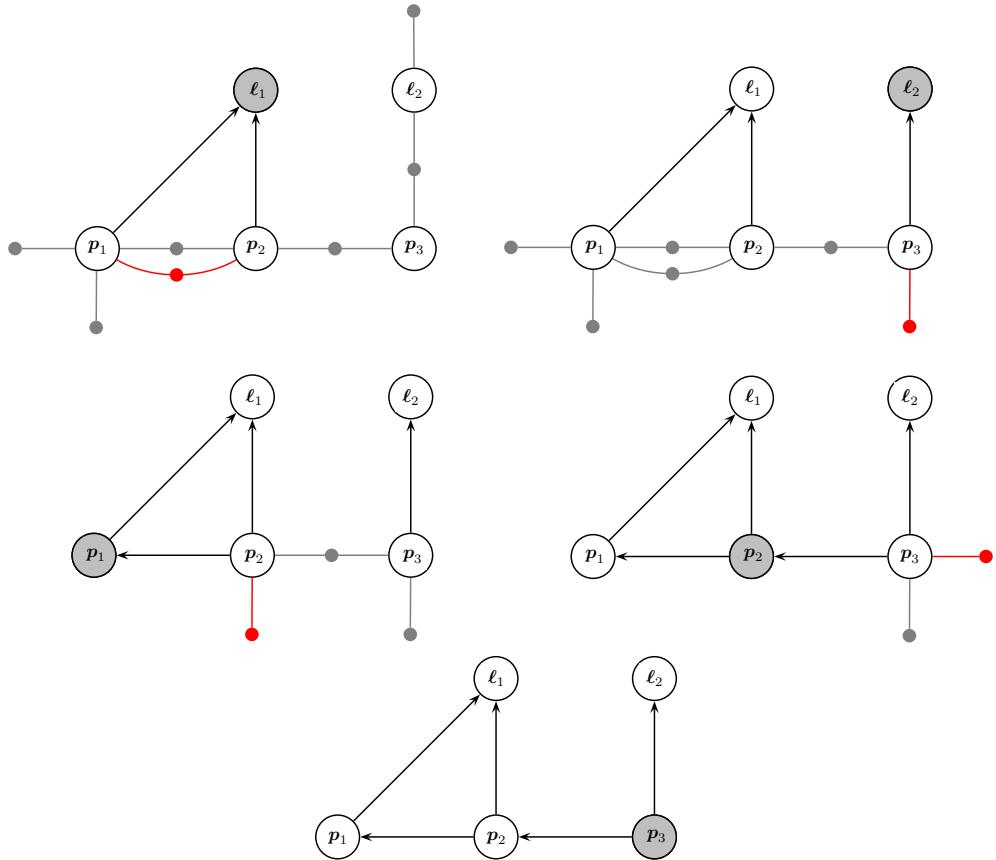
\includegraphics[width=\linewidth]{f367ec43cda5f3fdc37108cc58b8d68b91a0b1c5fd955c49cbdb6bffb688dce4.jpg}
\caption{图 1.10 玩具 SLAM 示例的变量消元：按 $\ell_1,\ell_2,p_1,p_2,p_3$ 的顺序，将图 1.3 的因子图转换为贝叶斯网络（右下）。}
\label{fig:f367ec43cda5f3fdc37108cc58b8d68b91a0b1c5fd955c49cbdb6bffb688dce4}
\end{figure}

因此，从 $\phi(\pmb x)$ 到 $p(\pmb x)$ 的完整分解，可以看作连续执行 $n$ 个局部分解步骤。当消除最后一个变量 $\pmb x_n$ 时，分隔集 $s_n$ 为空，因此得到的条件密度只是对 $\pmb x_n$ 的先验 $p(\pmb x_n)$。

对于玩具示例，一种可能的消元序列如图 1.10 所示，排序为 $\ell_1,\ell_2,p_1,p_2,p_3$。每一步中，被消元的变量以灰色阴影表示，分隔集 $s_j$ 上新生成的因子 $\tau(s_j)$ 以红色表示。整体而言，变量消元算法将因子图 $\phi(\ell_1,\ell_2,p_1,p_2,p_3)$ 分解为图 1.10（右下）的贝叶斯网络，对应的分解为

\begin{equation}
p \left(\ell_ {1}, \ell_ {2}, \boldsymbol {p} _ {1}, \boldsymbol {p} _ {2}, \boldsymbol {p} _ {3}\right) = p \left(\ell_ {1} \mid \boldsymbol {p} _ {1}, \boldsymbol {p} _ {2}\right) p \left(\ell_ {2} \mid \boldsymbol {p} _ {3}\right) p \left(\boldsymbol {p} _ {1} \mid \boldsymbol {p} _ {2}\right) p \left(\boldsymbol {p} _ {2} \mid \boldsymbol {p} _ {3}\right) p \left(\boldsymbol {p} _ {3}\right).\tag{1.44}
\end{equation}

\subsection{线性高斯消元}

在线性测量函数和加性正态分布噪声的情况下，变量消元算法等价于稀疏矩阵分解；稀疏 Cholesky 分解和 QR 分解都是该通用算法的特例。

如前所述，消元算法逐个处理变量。对于每个变量 $\boldsymbol\Delta_{\boldsymbol{\mathcal{X}}_j}$，移除与之相邻的所有因子 $\phi_i(\pmb x_i)$，并形成中间乘积因子 $\psi(\pmb x_j,\pmb s_j)$。只需将所有矩阵 $A_i$ 累积到一个更大的分块矩阵 $\bar A_j$ 中即可：

\begin{equation}
\psi(\boldsymbol {x} _ {j}, \boldsymbol {s} _ {j}) \leftarrow \prod_ {i \in \mathcal {N} _ {j}} \phi_ {i} (\boldsymbol {x} _ {i})\tag{1.45a}
\end{equation}

\begin{equation}
= \exp \left(- \frac {1}{2} \sum_ {i} \| \boldsymbol {A} _ {i} \boldsymbol {x} _ {i} - \boldsymbol {b} _ {i} \| _ {2} ^ {2}\right)\tag{1.45b}
\end{equation}

\begin{equation}
= \exp \left(- \frac {1}{2} \left\| \bar {\boldsymbol {A}} _ {j} [ \boldsymbol {x} _ {j}; \boldsymbol {s} _ {j} ] - \bar {\boldsymbol {b}} _ {j} \right\| _ {2} ^ {2}\right),\tag{1.45c}
\end{equation}

其中，新的右端项向量 $\bar{\boldsymbol b}_j$ 堆叠了所有 $\boldsymbol b_i$；符号 $[\cdot;\cdot]$ 表示按列（垂直）堆叠。

考虑在玩具示例中消去变量 $\ell_1$。与它相邻的因子为 $\phi_4,\phi_7,\phi_8$，从而诱导出分隔集 $\pmb s_1=[\pmb p_1;\pmb p_2]$。乘积因子等于

\begin{equation}
\psi \left(\boldsymbol {\ell} _ {1}, \boldsymbol {p} _ {1}, \boldsymbol {p} _ {2}\right) = \exp \left(- \frac {1}{2} \left\| \bar {\boldsymbol {A}} _ {1} [ \boldsymbol {\ell} _ {1}; \boldsymbol {p} _ {1}; \boldsymbol {p} _ {2} ] - \bar {\boldsymbol {b}} _ {1} \right\| _ {2} ^ {2}\right),\tag{1.46}
\end{equation}

其中

\begin{equation}
\bar {\boldsymbol {A}} _ {1} \triangleq \left[ \begin{array}{c c c} \boldsymbol {A} _ {4 1} & & \\ \boldsymbol {A} _ {7 1} & \boldsymbol {A} _ {7 3} & \\ \boldsymbol {A} _ {8 1} & & \boldsymbol {A} _ {8 4} \end{array} \right], \qquad \bar {\boldsymbol {b}} _ {1} \triangleq \left[ \begin{array}{c} \boldsymbol {b} _ {4} \\ \boldsymbol {b} _ {7} \\ \boldsymbol {b} _ {8} \end{array} \right].\tag{1.47}
\end{equation}

观察图 1.7 的稀疏雅可比矩阵，这相当于取出第一列中存在非零分块的那些分块行，也就是与 $\ell_1$ 相邻的三个因子。

接下来可以用多种方式对乘积 $\psi(\pmb x_j,\pmb s_j)$ 进行分解。这里讨论 QR 变体，因为它与线性化因子的联系更加直接。具体而言，与乘积因子 $\psi(\pmb x_j,\pmb s_j)$ 对应的增广矩阵 $[\bar A_j|\bar b_j]$ 可使用部分 QR 分解 \textsuperscript{[389]} 重写为

\begin{equation}
[ \bar {\boldsymbol {A}} _ {j} | \bar {\boldsymbol {b}} _ {j} ] = \boldsymbol {Q} \left[ \begin{array}{c c c} \boldsymbol {R} _ {j} & \boldsymbol {T} _ {j} & \boldsymbol {d} _ {j} \\ & \tilde {\boldsymbol {A}} _ {\tau} & \tilde {\boldsymbol {b}} _ {\tau} \end{array} \right],\tag{1.48}
\end{equation}

其中 $R_j$ 是上三角矩阵。由此，$\psi(\pmb x_j,\pmb s_j)$ 可以分解为

\begin{equation}
\begin{array}{l} \psi (\boldsymbol {x} _ {j}, \boldsymbol {s} _ {j}) = \exp \left\{- \frac {1}{2} \left\| \bar {\boldsymbol {A}} _ {j} [ \boldsymbol {x} _ {j}; \boldsymbol {s} _ {j} ] - \bar {\boldsymbol {b}} _ {j} \right\| _ {2} ^ {2} \right\} \\ = \exp \left\{- \frac {1}{2} \left\| \boldsymbol {R} _ {j} \boldsymbol {x} _ {j} + \boldsymbol {T} _ {j} \boldsymbol {s} _ {j} - \boldsymbol {d} _ {j} \right\| _ {2} ^ {2} \right\} \exp \left\{- \frac {1}{2} \left\| \tilde {\boldsymbol {A}} _ {\tau} \boldsymbol {s} _ {j} - \tilde {\boldsymbol {b}} _ {\tau} \right\| _ {2} ^ {2} \right\} \\ = p (\boldsymbol {x} _ {j} | \boldsymbol {s} _ {j}) \tau (\boldsymbol {s} _ {j}), \end{array}\tag{1.49a}
\end{equation}

\begin{equation}
\left\| \bar {\boldsymbol {A}} _ {j} [ \boldsymbol {x} _ {j}; \boldsymbol {s} _ {j} ] - \bar {\boldsymbol {b}} _ {j} \right\| _2^2 = \left\| \boldsymbol {R}_j\boldsymbol{x}_j+\boldsymbol{T}_j\boldsymbol{s}_j-\boldsymbol{d}_j\right\|_2^2 + \left\|\tilde{\boldsymbol A}_\tau\boldsymbol{s}_j-\tilde{\boldsymbol b}_\tau\right\|_2^2.\tag{1.49b}
\end{equation}

其中利用了旋转矩阵 $Q$ 不会改变相关范数值这一事实。

在玩具示例中，图 1.11 展示了消去第一个变量 $\ell_1$（其分隔集为 $[p_1;p_2]$）的结果。图中同时展示了因子图上的操作，以及对图 1.7 稀疏雅可比矩阵的相应影响（省略右端项）。分界线以上的部分对应正在形成的稀疏上三角矩阵 $R$；矩阵的新贡献用蓝色表示，新生成的因子用红色表示。为完整起见，图 1.12 展示了其余四个变量消元步骤，给出了 QR 分解如何在一个小型示例上端到端执行。最后一步展示了生成的贝叶斯网络与稀疏上三角因子 $R$ 之间的等价性。

\begin{figure}[htbp]
\centering
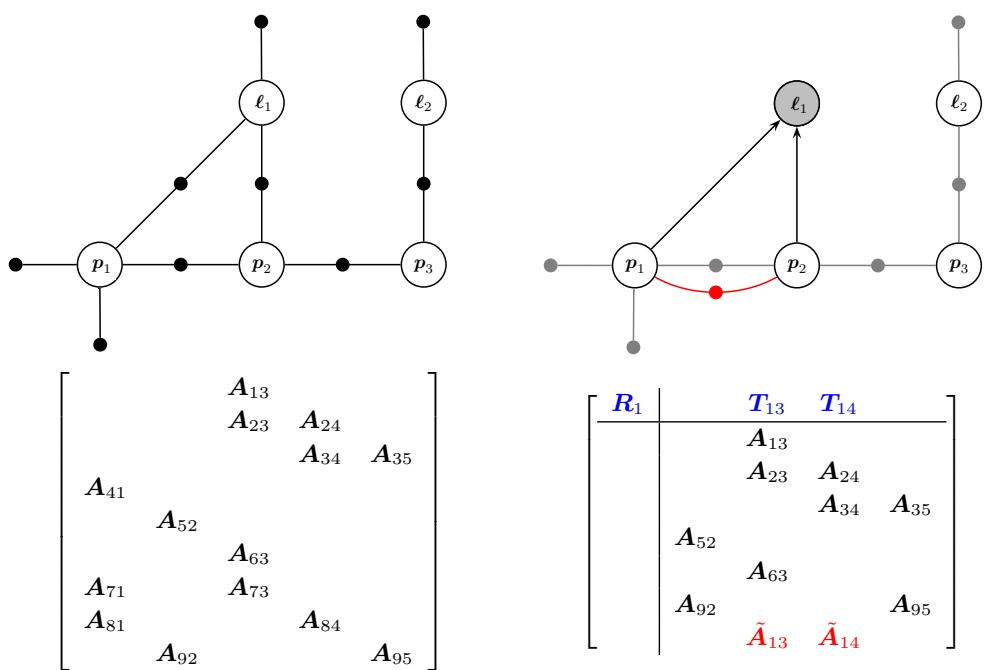
\includegraphics[width=\linewidth]{7f7da02ffac9b2ac7ca9019d72b500da0d139492bdb2841af98e305211d9b176.jpg}
\caption{图 1.11 将变量 $\ell_1$ 消元作为一次部分稀疏分解步骤。}
\label{fig:7f7da02ffac9b2ac7ca9019d72b500da0d139492bdb2841af98e305211d9b176}
\end{figure}

使用部分 QR 分解消除单个变量的完整消元算法，等价于稀疏 QR 分解。由于上面的处理考虑了多维变量 $\pmb x_j\in\mathbb R^{n_j}$，因此实际上这是多前沿 QR 分解 \textsuperscript{[288]} 的一个实例：每次同时消除多个标量变量，这有利于提高处理器利用率。在这里，标量变量按其在推断问题中的语义进行分组；而稀疏线性代数程序通常会按最大化计算效率的目标分析并分组问题。许多情况下，这两种策略高度一致。

\begin{figure}[htbp]
\centering
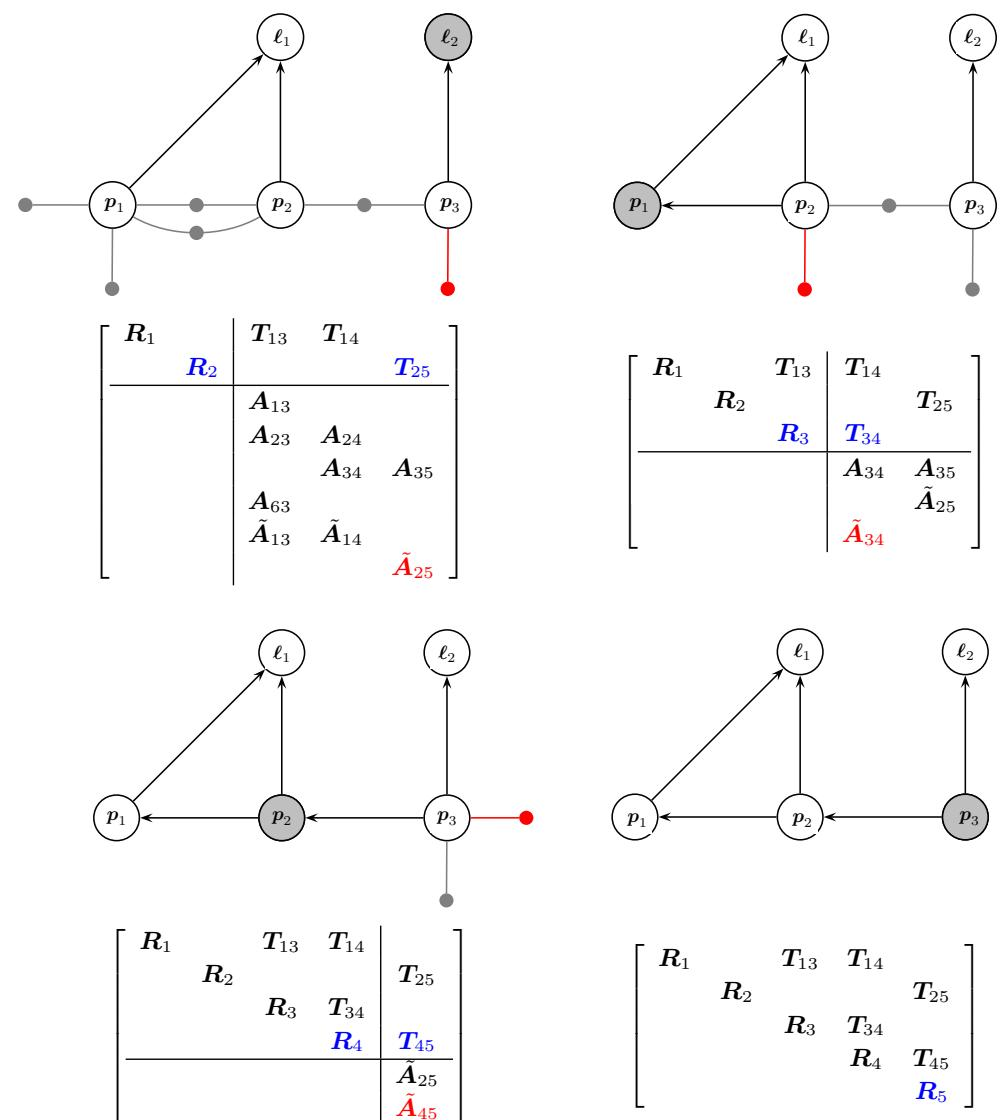
\includegraphics[width=\linewidth]{e2e8d95287a0da35908e51410277a99b2c009af7c8e501191f52e42f89f6f4b6.jpg}
\caption{图 1.12 玩具示例中剩余的消元步骤，完成一次完整 QR 分解。右下角的最后一步展示了最终贝叶斯网络与稀疏 Cholesky 因子 $R$ 的等价性。}
\label{fig:e2e8d95287a0da35908e51410277a99b2c009af7c8e501191f52e42f89f6f4b6}
\end{figure}

\subsection{作为贝叶斯网络的稀疏 Cholesky 因子}

变量消元与稀疏矩阵分解之间的等价性揭示了一个事实：与上三角矩阵关联的图模型就是贝叶斯网络！正如因子图是稀疏雅可比矩阵的图形化表示，贝叶斯网络揭示了 Cholesky 因子的稀疏结构。事后看来，这并不令人意外：贝叶斯网络是有向无环图（DAG），而这正对应矩阵的“上三角”性质。

此外，Cholesky 因子对应于高斯贝叶斯网络，即由线性高斯条件分布组成的贝叶斯网络。变量消元算法适用于一般密度；但当因子图只包含线性测量函数和高斯加性噪声时，得到的贝叶斯网络具有非常具体的形式。下面将讨论细节，以及在线性情形下如何求解 MAP 估计。

如前所述，与线性化非线性问题对应的高斯因子图，通过消元转化为密度 $p(\pmb x)$，其贝叶斯网络分解形式为

\begin{equation}
p (\boldsymbol {x}) = \prod_ {j} p (\boldsymbol {x} _ {j} | \boldsymbol {s} _ {j}).\tag{1.50}
\end{equation}

无论采用 QR 还是 Cholesky 变体，条件密度 $p(\pmb x_j|\pmb s_j)$ 都为

\begin{equation}
p (\boldsymbol {x} _ {j} | \boldsymbol {s} _ {j}) = k \exp \left(- \frac {1}{2} \| \boldsymbol {R} _ {j} \boldsymbol {x} _ {j} + \boldsymbol {T} _ {j} \boldsymbol {s} _ {j} - \boldsymbol {d} _ {j} \| _ {2} ^ {2}\right),\tag{1.51}
\end{equation}

这是关于已消元变量 $\pmb x_j$ 的线性高斯密度。事实上，有

\begin{equation}
\| \boldsymbol {R} _ {j} \boldsymbol {x} _ {j} + \boldsymbol {T} _ {j} \boldsymbol {s} _ {j} - \boldsymbol {d} _ {j} \| _ {2} ^ {2} = (\boldsymbol {x} _ {j} - \boldsymbol {\mu} _ {j}) ^ {\top} \boldsymbol {R} _ {j} ^ {\top} \boldsymbol {R} _ {j} (\boldsymbol {x} _ {j} - \boldsymbol {\mu} _ {j}) \stackrel {{\Delta}} {{=}} \| \boldsymbol {x} _ {j} - \boldsymbol {\mu} _ {j} \| _ {\Sigma_ {j}} ^ {2},\tag{1.52}
\end{equation}

其中，均值 $\pmb\mu_j=\pmb R_j^{-1}(\pmb d_j-\pmb T_j\pmb s_j)$ 线性依赖于分隔集 $s_j$，协方差矩阵为 $\pmb\Sigma_j=(\pmb R_j^\top\pmb R_j)^{-1}$。因此，归一化常数为 $k=|2\pi\Sigma_j|^{-1/2}$。

消元步骤完成后，使用回代获得每个变量的 MAP 估计。如图 1.12 所示，最后被消元的变量不依赖于任何其他变量，因此可以直接从贝叶斯网络中提取该变量的 MAP 估计。按照消元顺序的逆序继续进行时，每个条件分布的所有分隔变量都将在前面的步骤中获得，从而可以计算当前前端变量的估计。

在每一步中，变量 $\boldsymbol\Delta_{\boldsymbol{\mathcal{X}}_j}$ 的 MAP 估计就是条件均值：

\begin{equation}
\pmb {x} _ {j} ^ {*} = \pmb {R} _ {j} ^ {- 1} (\pmb {d} _ {j} - \pmb {T} _ {j} \pmb {s} _ {j} ^ {*}),\tag{1.53}
\end{equation}

因为到此时，分隔集 $s_j$ 的 MAP 估计 $s_j^*$ 已经完全确定。

\section{增量式 SLAM}

在增量式 SLAM 场景中，机器人穿行环境并不断接收新测量时，我们希望及时（或至少以固定间隔）计算最优轨迹和地图。一种方式是用新测量更新最近一次矩阵分解，复用已经纳入先前全部测量的计算结果。在线性情况下，可以通过增量分解方法实现这一点，其稠密版本在 Golub 和 Van Loan \textsuperscript{[389]} 中有详细讨论。然而，矩阵分解作用于线性系统，而实际关心的大多数 SLAM 问题都是非线性的。采用增量矩阵分解时，如何在不重新分解完整矩阵的情况下执行增量式重新线性化，并不显然。为解决这个问题，我们再次借助图模型，引入一种新的图模型——贝叶斯树。随后将说明，如何在系统加入新测量和新状态时增量更新贝叶斯树，从而得到增量平滑与建图（iSAM）算法。

\subsection{贝叶斯树}

众所周知，在树结构图中的推断是高效的。相比之下，典型机器人问题对应的因子图包含许多环。不过，我们可以分两步构造树结构图模型：第一步，对因子图执行变量消元，得到具有特殊性质的贝叶斯网络；第二步，利用该特殊性质，找到该贝叶斯网络中各个团之间的树结构。

通过因子图运行消元算法得到的贝叶斯网络具有一个特殊性质：它是弦图（chordal graph），即任意长度大于 3 的无向环都包含一条弦，也就是连接环上两个非相邻顶点的边。在人工智能和机器学习领域，弦图更常称为三角化图。由于它仍然是贝叶斯网络，其联合密度 $p(\pmb x)$ 可以在各个变量 $\boldsymbol\Delta_{\boldsymbol{\mathcal{X}}_j}$ 上分解：

\begin{equation}
p (\boldsymbol {x}) = \prod_ {j} p (\boldsymbol {x} _ {j} | \boldsymbol {\pi} _ {j}),\tag{1.54}
\end{equation}

其中，$\pi_j$ 是 $\boldsymbol\Delta_{\boldsymbol{\mathcal{X}}_j}$ 的父节点。不过，尽管贝叶斯网络是弦图，在变量层面它仍是一个非平凡图：既不是链式结构，也不是树结构。图 1.10 最后一步给出了当前玩具 SLAM 示例的弦贝叶斯网络；其中存在无向环 $\pmb p_1-\pmb p_2-\pmb\ell_1$，说明它不具备树结构。

通过识别这个弦图中的团，可以将贝叶斯网络改写为贝叶斯树。我们引入这种新的树结构图模型，用来捕捉贝叶斯网络中的团结构。贝叶斯网络中的团之所以能构成一棵树，并不显然；这是弦性质的结果，这里不再证明。将所有这些团列在一棵无向树上，就得到团树，在人工智能和机器学习中也称为连接树。贝叶斯树只是团树的有向版本，同时保留了消元顺序的信息。

更形式化地说，贝叶斯树是一棵有向树，其节点表示底层弦贝叶斯网络中的团 $c_k$。具体而言，每个节点定义一个条件密度 $p(f_k|s_k)$，其中分隔集 $\pmb s_k$ 是团 $c_k$ 与其父团 $\varpi_k$ 的交集 $c_k\cap\varpi_k$。前端变量 $\pmb f_k$ 是剩余变量，即 $\pmb f_k\triangleq\pmb c_k\setminus\pmb s_k$。记号上，将一个团写成 $\pmb c_k=\pmb f_k:\pmb s_k$。由贝叶斯树定义的变量联合密度为

\begin{equation}
p (\boldsymbol {x}) = \prod_ {k} p (\boldsymbol {f} _ {k} | \boldsymbol {s} _ {k}).\tag{1.55}
\end{equation}

对于根节点 $f_r$，分隔集为空，即它只是根变量上的简单先验 $p(f_r)$。按照贝叶斯树的定义，团 $c_k$ 的分隔集 $\pmb s_k$ 始终是其父团 $\varpi_k$ 的子集，因此图中的有向边与贝叶斯网络中的语义相同：表示条件依赖。

与当前玩具 SLAM 问题（图 1.3）关联的贝叶斯树如图 1.13 所示。根团 $\pmb c_1=\{\pmb p_2,\pmb p_3\}$（蓝色）由 $p_2$ 和 $p_3$ 组成，并与另外两个团相交：绿色团 $\pmb c_2=\{\pmb\ell_1,\pmb p_1\}:\pmb p_2$，以及红色团 $c_3=\{\ell_2\}:\{p_3\}$。颜色还表示平方根信息矩阵 $R$ 的行如何映射到不同团，以及贝叶斯树如何捕捉它们之间的独立关系。例如，绿色和红色行只在属于根团的变量上相交，正如预期。

\subsection{更新贝叶斯树}

增量推断可以看作对贝叶斯树进行简单编辑。这种视角能够更好地解释和理解原本抽象的增量矩阵分解过程，也允许我们以贝叶斯树的形式存储和计算平方根信息矩阵，从而得到具有明确语义的稀疏存储结构。

为了增量更新贝叶斯树，我们有选择地将贝叶斯树的一部分转换回因子图形式。加入新测量时，相当于加入一个新因子；例如，涉及两个变量的测量会产生新的二元因子 $\phi(\pmb x_j,\pmb x_{j'})$。此时，只有连接包含 $\pmb x_j$ 和 $\pmb x_{j'}$ 的团与根节点的路径会受到影响。这些团下方的子树不受影响，其他不包含这两个变量的子树也不受影响。因此，更新贝叶斯树时，只需将受影响部分转换回因子图，加入与新测量关联的新因子，然后使用任意方便的消元顺序重新消元这个临时因子图，构造新的贝叶斯树，最后重新接回未受影响的子树。

之所以只有树的上部受到影响，可以从贝叶斯树的两个重要性质理解。第一，贝叶斯树由弦贝叶斯网络按照消元顺序的逆序构成，因此每个团中的变量通过消去子团来收集来自子团的信息；任何团中的信息只会向上方根节点传播。第二，一个因子只有在与它相连的第一个变量被消去时才会进入消元过程。结合这两个性质可知，新因子不会影响那些不是其变量后继的变量。但是，如果一个因子涉及分别沿不同（即相互独立）路径连接到根的变量，那么为了表达它们之间新产生的依赖关系，就必须重新消去这些路径。

图 1.14 展示了如何在典型 SLAM 示例中应用这些增量分解/推断步骤。在该示例中，我们在 $\pmb p_1$ 与 $\pmb p_3$ 之间加入一个新因子，因此只影响树的左分支（左上图红色虚线标记部分）。随后构造右上图所示因子图：为每个团密度 $p(p_2,p_3)$ 和 $p(\ell_1,p_1|p_2)$ 建立因子，并加入新因子 $f(p_1,p_3)$。右下图显示了按 $\ell_1,p_1,p_2,p_3$ 顺序消元后得到的图。最后，左下图给出重新组装的贝叶斯树，它由消元图得到的新树和原始贝叶斯树中未受影响的团（绿色）构成。

图 1.15 展示了一个小型 SLAM 序列的贝叶斯树示例，数据取自 Olson 等人 \textsuperscript{[824]} 著名的“曼哈顿世界”模拟序列第 400 步。机器人探索环境时，新测量通常只影响树的一小部分，因此只需重新计算这些部分。

\subsection{增量平滑与建图}

将上述内容结合起来，并考虑重新线性化等实际问题，就得到一种最先进的增量式非线性机器人 MAP 估计方法 iSAM。第一个版本 iSAM1 \textsuperscript{[531]} 使用了 Golub 和 Van Loan \textsuperscript{[389]} 的增量矩阵分解方法，但它以次优方式处理线性化：定期在完整因子图上进行线性化，和/或在矩阵填充变得难以处理时进行线性化。第二个版本 iSAM2 使用贝叶斯树表示后验密度 \textsuperscript{[534]}；随后如上所述，每当接收到新测量，就通过贝叶斯树增量更新来处理。

重新消除受影响团时，应该采用怎样的变量排序？只有贝叶斯树受影响部分中的变量需要更新。一种策略是在受影响变量上局部应用 COLAMD。但还可以做得更好：将最近访问的变量强制放到排序末端，即放入根团。对于这种增量变量排序策略，可以使用约束 COLAMD 算法 \textsuperscript{[241]}。它既能将最近访问的变量置于末端，又能保持总体上良好的排序。通常，后续更新只会影响树的一小部分，因此除大型回环外，大多数情况下都能高效完成。

更新树之后，还需要更新解。贝叶斯树中的回代从不依赖其他变量的根节点开始，逐步向叶节点进行。不过，通常不必重新计算所有变量的解：树的局部更新往往不会影响远处的变量。相反，在每个团处检查向下传播的变量估计变化，当该变化低于一个很小的阈值时即可停止。

引入贝叶斯树的动机，是增量求解非线性优化问题。为此，我们有选择地对包含某些变量的因子重新线性化，前提是这些变量偏离线性化点超过一个很小的阈值。与上面的树修改不同，此时必须重新处理包含受影响变量的所有团，不仅包括它们作为前端变量的情形，也包括作为分隔变量的情形。这样会影响树的更大部分，但在大多数情况下仍显著低于重建整棵树的代价。此外，我们还需要回到原始因子，而不能直接把团转换成因子图，这要求在消元时缓存某些量。完整的增量非线性算法 iSAM2 可参见 \textsuperscript{[534]}。

iSAM1 和 iSAM2 已成功应用于许多不同的机器人估计问题，其中变量之间存在非平凡约束，变量数量可达数百万；后续章节还会进一步讨论。两种算法都在 GTSAM 库中实现，代码见 https://github.com/borglab/gtsam。

\section{延伸阅读与近期趋势}

希望深入了解因子图的读者，可以参阅 Dellaert 等人 \textsuperscript{[255]} 的长篇文章。由于篇幅所限，本章相对简略，并弱化了一些高级概念，以尽可能降低入门门槛。不过，因子图和一般变量消元算法都非常强大，值得系统掌握。之后建议阅读 Kaess 等人 \textsuperscript{[534]}，进一步理解贝叶斯树这一支撑 GTSAM 等现代求解器的核心概念。

如今，因子图范式可以处理流形上的状态变量，融合多种传感器，处理离群测量，甚至纳入深度学习方法的输出。本手册的其余部分将大量讨论这些趋势，读者可继续阅读以了解详情。

\chapter{高级状态变量表示}

\textbf{作者：} Timothy Barfoot、Frank Dellaert、Michael Kaess、Jose Luis Blanco-Claraco

上一章详细介绍了如何采用因子图范式建立并求解 SLAM 问题。为便于说明，我们有意避开了所估计状态变量的一些细节。本章重新审视状态变量的性质，并介绍现代 SLAM 形式化中普遍存在的两个重要主题。

首先，我们需要更好的工具来处理带有特定约束的状态变量；这些约束为变量定义了一个流形，因此在优化时必须特别处理。SLAM 中存在许多流形，最常见的是与机器人旋转相关的流形（尤其是三维旋转，但平面旋转也属于这一类）。

其次，状态变量的另一个方面来自时间本身的性质。上一章隐式地假设机器人以离散时间步在世界中运动。本章将引入轨迹的平滑连续时间表示，并讨论它们如何与因子图形式完全兼容。我们以 Barfoot \textsuperscript{[47]} 为主要参考，并采用 Sola 等人 \textsuperscript{[1022]} 的简化记号。

\subsection{流形上的优化}

在某些机器人问题中，可以使用向量值未知量；但在大多数实际场景中，我们必须处理三维旋转以及其他非向量流形。粗略地说，流形是一个拓扑闭合的曲面（例如圆的周长或球面）；重要的是，在每个点附近，流形局部上都类似于欧氏空间。处理流形需要更精密的数学工具，以考虑其特殊结构。本节讨论如何在流形上执行优化，这将在上一章向量空间优化框架的基础上展开。作为示例，图 2.1 对球面流形 $\mathcal{M}$ 及其切空间 $T_x\mathcal{M}$ 进行了可视化；切空间可作为 $x\in\mathcal{M}$ 处用于优化的局部坐标系。

\begin{figure}[htbp]
\centering
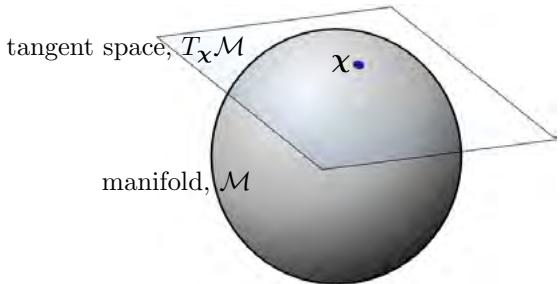
\includegraphics[width=\linewidth]{bbe04e3dd68402335deae02f97a01ba9bd5413b1b433cd0d96e4948fd713088a.jpg}
\caption{图 2.1 对于球面流形 $\mathcal{M}$，$T_x\mathcal{M}$ 是局部切平面；配合局部基，可以定义局部坐标。}
\label{fig:bbe04e3dd68402335deae02f97a01ba9bd5413b1b433cd0d96e4948fd713088a}
\end{figure}

\subsection{旋转与位姿}

在 SLAM 语境中可以讨论许多流形，但最常见的两类用于表示旋转和位姿。旋转通常发生在二维（平面）或三维空间中，因此将旋转流形称为特殊正交群 $\mathrm{SO}(d)$，其中 $d=2$ 或 $3$。平面旋转矩阵 $R_a^b\in\mathrm{SO}(2)$ 的形式为

\begin{equation}
\boldsymbol {R} _ {a} ^ {b} = \left[ \begin{array}{c c} \cos \theta & - \sin \theta \\ \sin \theta & \cos \theta \end{array} \right],\tag{2.1}
\end{equation}

其中 $\theta\in\mathbb{R}$ 是旋转角，也是该情形下唯一的自由度。此外，$R_a^b$ 可将参考坐标系 $\mathcal{F}^a$ 中表示的二维向量（例如路标）旋转到 $\mathcal{F}^b$ 中：$\ell^b=R_a^b\ell^a$。

三维旋转矩阵 $R_a^b\in\mathrm{SO}(3)$ 同样用于在两个坐标系之间旋转向量，只是此时向量处于三维空间。三维旋转矩阵有 9 个元素，但只有 3 个自由度（例如滚转、俯仰和偏航）。二维和三维旋转矩阵都必须满足约束

\begin{equation*}
\pmb { R } _ { a } ^ { b \top } \pmb { R } _ { a } ^ { b } = \mathbf { I }, \qquad \det (\boldsymbol {R} _ {a} ^ {b})=1,
\end{equation*}

以适当地限制自由度。

机器人的位姿同时包含旋转变量 $R_a^b\in\mathrm{SO}(d)$ 和平移变量 $\pmb t_a^b\in\mathbb{R}^d$，总共有 $3(d-1)$ 个自由度。有时我们分别跟踪这两类量，并使用 $\{R_a^b,\pmb t_a^b\}\in\mathrm{SO}(d)\times\mathbb{R}^d$ 表示位姿。另一种方式是将它们组合成一个 $(d+1)\times(d+1)$ 的变换矩阵：

\begin{equation}
\boldsymbol {T} _ {a} ^ {b} = \left[ \begin{array}{c c} \boldsymbol {R} _ {a} ^ {b} & \boldsymbol {t} _ {a} ^ {b} \\ \boldsymbol {0} & 1 \end{array} \right].\tag{2.2}
\end{equation}

所有这类变换矩阵组成的流形称为特殊欧氏群 $\operatorname{SE}(d)$，其中 $d=2$ 表示平面运动，$d=3$ 表示三维运动。使用 $\operatorname{SE}(d)$ 的好处是，可以通过一次矩阵乘法同时对路标进行旋转和平移：

\begin{equation}
\underbrace {\left[ \begin{array}{c} \boldsymbol {\ell} ^ {b} \\ 1 \end{array} \right]} _ {\tilde {\boldsymbol {\ell}} ^ {b}} = \underbrace {\left[ \begin{array}{c c} \boldsymbol {R} _ {a} ^ {b} & \boldsymbol {t} _ {a} ^ {b} \\ \boldsymbol {0} & 1 \end{array} \right]} _ {\boldsymbol {T} _ {a} ^ {b}} \underbrace {\left[ \begin{array}{c} \boldsymbol {\ell} ^ {a} \\ 1 \end{array} \right]} _ {\tilde {\boldsymbol {\ell}} ^ {a}},\tag{2.3}
\end{equation}

其中 $\tilde\ell$ 是路标的齐次表示。

由于旋转矩阵和变换矩阵的形式受到约束，它们并不是向量。例如，不能简单地将两个旋转矩阵相加，并期望结果仍是有效的旋转矩阵。不过，$\mathrm{SO}(d)$ 和 $\operatorname{SE}(d)$ 都属于具有额外有用结构的流形，即\textbf{矩阵 Lie 群}。我们可以利用这种结构，在因子图 SLAM 中继续执行无约束 MAP 优化（参见 Dellaert 等人 \textsuperscript{[255]}、Boumal \textsuperscript{[106]} 或 Barfoot \textsuperscript{[47]}）。关于机器人中的 Lie 群，可参考 Chirikjian 和 Kyatkin \textsuperscript{[207]} 以及 Chirikjian \textsuperscript{[205, 206]} 的经典工作。

\subsection{矩阵 Lie 群}

在 $\mathrm{SO}(d)$ 和 $\operatorname{SE}(d)$ 上执行优化的关键，是利用它们的群结构。例如，矩阵 Lie 群在矩阵乘法下封闭：若 $R_b^c,R_a^b\in\mathrm{SO}(d)$，则乘积也属于该群，且 $R_a^c=R_b^cR_a^b\in\mathrm{SO}(d)$。

矩阵 Lie 群还伴随一个非常有用的结构，称为 Lie 代数；它同时也是 Lie 群在单位元处的切空间。对我们而言，Lie 代数最重要的两个性质是：（i）它是一个向量空间，其维度等于对应 Lie 群的自由度数量；（ii）存在一个成熟的映射（矩阵指数）将 Lie 代数映射到 Lie 群。因此，可以从 Lie 代数元素相对容易地构造 Lie 群元素。例如，对于 SO(2)，暂时省略上下标，有

\begin{equation}
\boldsymbol {R} = \operatorname {Exp} (\theta) = \exp (\theta^ {\wedge}) = \sum _ {n = 0} ^ {\infty} \frac {1}{n !} (\theta^ {\wedge}) ^ {n} = \left[ \begin{array}{c c} \cos \theta & - \sin \theta \\ \sin \theta & \cos \theta \end{array} \right] \in \operatorname {SO} (2),\tag{2.4}
\end{equation}

其中

\begin{equation}
\theta^ {\wedge} = \left[ \begin{array}{c c} 0 & - \theta \\ \theta & 0 \end{array} \right], \qquad \theta \in \mathbb {R}.\tag{2.5}
\end{equation}

量 $\theta^\wedge$ 属于 Lie 代数 $\mathrm{so}(2)$，通过矩阵指数 $\exp(\cdot)$ 映射为 Lie 群元素 $R$。反向也可以使用矩阵对数和 vee 算子完成：$\theta=\operatorname{Log}(R)=(\log R)^\vee$。vee 算子 $(\cdot)^\vee$ 是 wedge 算子 $(\cdot)^\wedge$ 的逆。

\begin{figure}[htbp]
\centering
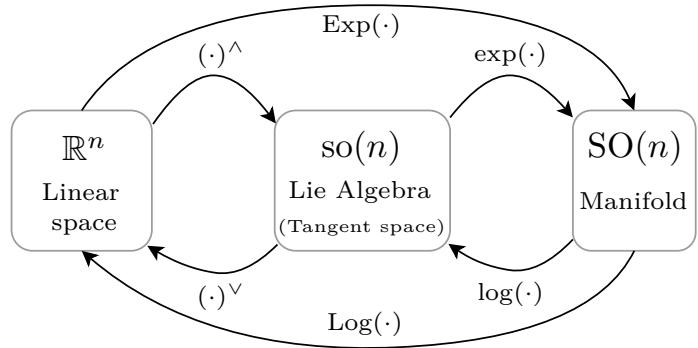
\includegraphics[width=\linewidth]{804afd145bba6076b0a4f9b2a7a50f021aa403f602569619e3b9cc5ac1ed7830.jpg}
\caption{图 2.2 本章记号概览：wedge 算子 $(\cdot)^\wedge$ 与 vee 算子 $(\cdot)^\vee$，指数映射 $\exp(\cdot)$ 与对数映射 $\log(\cdot)$，以及便捷记号 $\operatorname{Exp}(\cdot)=\exp((\cdot)^\wedge)$ 和 $\operatorname{Log}(\cdot)=(\log(\cdot))^\vee$。图中以 $\mathrm{SO}(n)$ 为例，但这些算子对其他流形同样定义。}
\label{fig:804afd145bba6076b0a4f9b2a7a50f021aa403f602569619e3b9cc5ac1ed7830}
\end{figure}

每个矩阵 Lie 群都有自己的线性 wedge 算子，用于从相应维度的标准向量空间构造 Lie 代数元素。对于 $\mathrm{SO}(3)$，它是反对称算子：

\begin{equation}
\boldsymbol {R} = \operatorname{Exp} (\boldsymbol {\theta}) = \exp (\boldsymbol {\theta} ^ {\wedge}) = \sum_ {n = 0} ^ {\infty} \frac {1}{n !} \boldsymbol {\theta} ^ {\wedge n} \in \mathrm{SO} (3),\tag{2.6a}
\end{equation}

\begin{equation}
\boldsymbol {\theta} ^ {\wedge} = \left[ \begin{array}{c c c} 0 & - \theta_ {3} & \theta_ {2} \\ \theta_ {3} & 0 & - \theta_ {1} \\ - \theta_ {2} & \theta_ {1} & 0 \end{array} \right] \in \operatorname{so} (3), \quad \boldsymbol {\theta} = \left[ \begin{array}{c} \theta_ {1} \\ \theta_ {2} \\ \theta_ {3} \end{array} \right] \in \mathbb {R} ^ {3}.\tag{2.6b}
\end{equation}

对于 $\operatorname{SE}(d)$，可写成

\begin{equation}
\boldsymbol {T} = \mathrm{Exp} (\boldsymbol {\xi}) = \mathrm{exp} (\boldsymbol {\xi} ^ {\wedge}) \in \mathrm{SE} (d),\tag{2.7a}
\end{equation}

\begin{equation}
\boldsymbol {\xi} ^ {\wedge} = \left[ \begin{array}{c c} \boldsymbol {\theta} ^ {\wedge} & \boldsymbol {\rho} \\ \mathbf {0} & 0 \end{array} \right] \in \operatorname{se} (d), \quad \boldsymbol {\xi} = \left[ \begin{array}{c} \boldsymbol {\rho} \\ \boldsymbol {\theta} \end{array} \right] \in \mathbb {R} ^ {3 (d - 1)}, \quad \boldsymbol {\theta} \in \mathbb {R} ^ {2 d - 3}, \quad \boldsymbol {\rho} \in \mathbb {R} ^ {d}.\tag{2.7b}
\end{equation}

这里 $d=2$（平面）或 $3$（三维）。注意，wedge 算子的具体版本可以由输入向量的大小确定。对于这里讨论的每个矩阵 Lie 群，Lie 代数与 Lie 群之间的映射还存在众所周知的闭式表达式，可以替代矩阵指数的无穷级数形式 \textsuperscript{[47]}。

\subsection{Lie 群优化}

建立矩阵 Lie 群之后，就可以利用它们将非线性最小二乘项“线性化”，从而执行 MAP 推断。回顾第 1.3.1 节，我们仍然要线性化测量函数 $\pmb h_i(\cdot)$，只是其输入现在可能包含 Lie 群元素。

例如，假设 $\pmb h_i(\cdot)$ 是一个相机模型，它接收在相机坐标系中表示的齐次路标 $\tilde\ell_i^c$，并返回图像中的像素坐标 $z_i\in\mathbb{R}^2$。传感器生成模型可写为

\begin{equation}
\boldsymbol {z} _ {i} = \boldsymbol {h} _ {i} \left(\boldsymbol {T} _ {w} ^ {c} \tilde {\ell} _ {i} ^ {w}\right) + \boldsymbol {\eta} _ {i}.\tag{2.8}
\end{equation}

其中，$\pmb T_w^c\in\mathrm{SE}(3)$ 是相对于相机坐标系的世界坐标系位姿，$\tilde\ell_i^w$ 是在世界坐标系中表示的齐次路标，$\pmb\eta_i$ 是通常的传感器噪声。我们希望求解

\begin{equation}
\boldsymbol {T} _ {w} ^ {c ^ {*}} = \underset {\boldsymbol {T} _ {w} ^ {c}} {\arg \min} \sum_ {i} \left\| \boldsymbol {z} _ {i} - \boldsymbol {h} _ {i} \left(\boldsymbol {T} _ {w} ^ {c} \tilde {\ell} _ {i} ^ {w}\right) \right\| _ {\boldsymbol {\Sigma} _ {i}} ^ {2},\tag{2.9}
\end{equation}

这就是透视 n 点（perspective-n-point，PNP）问题。本例假设世界坐标系中的路标位置已知；当然，在 SLAM 中也可能需要同时估计它们。

为了线性化传感器模型，利用 Lie 代数产生位姿的扰动：

\begin{equation}
\pmb {T} _ {w} ^ {c} = \pmb {T} _ {w} ^ {c ^ {0}} \mathrm{Exp} (\pmb {\xi}).\tag{2.10}
\end{equation}

这里 $\pmb\xi\in\mathbb{R}^6$ 产生一个“小的”位姿变化，用于扰动初始猜测 $\pmb T_w^{c^0}\in\mathrm{SE}(3)$。也常用简写记号

\begin{equation}
\pmb {T} _ {w} ^ {c} = \pmb {T} _ {w} ^ {c ^ {0}} \oplus \pmb {\xi},\tag{2.11}
\end{equation}

它是式（2.10）的缩写。由于群的封闭性，这两个量的乘积必然属于 SE(3)。使用 Lie 代数定义位姿扰动，可以将其维度限制为三维位姿的实际自由度数量，从而在优化过程中无需额外引入约束。

还可以用矩阵指数的级数形式近似扰动位姿：

\begin{equation}
\boldsymbol {T} _ {w} ^ {c} \approx \boldsymbol {T} _ {w} ^ {c ^ {0}} \left(\mathbf {I} + \boldsymbol {\xi} ^ {\wedge}\right).\tag{2.12}
\end{equation}

其中只保留了关于 $\pmb\xi$ 的一次项。将式（2.12）代入测量函数（式 2.8），得到

\begin{equation}
\boldsymbol {z} _ {i} \approx \boldsymbol {h} _ {i} \left(\boldsymbol {T} _ {w} ^ {c ^ {0}} \left(\mathbf {I} + \boldsymbol {\xi} ^ {\wedge}\right) \tilde {\ell} _ {i} ^ {w}\right) + \boldsymbol {\eta} _ {i}.\tag{2.13}
\end{equation}

利用齐次点的线性算子 $\odot$，还可写成

\begin{equation}
\boldsymbol {z} _ {i} \approx \boldsymbol {h} _ {i} \left(\boldsymbol {T} _ {w} ^ {c ^ {0}} \tilde {\ell} _ {i} ^ {w} + \boldsymbol {T} _ {w} ^ {c ^ {0}} \tilde {\ell} _ {i} ^ {w ^ {\odot}} \boldsymbol {\xi}\right) + \boldsymbol {\eta} _ {i},\tag{2.14}
\end{equation}

其中

\begin{equation}
\tilde {\boldsymbol {\ell}} ^ {\odot} = \left[ \begin{array}{c} \boldsymbol {\ell} \\ 1 \end{array} \right] ^ {\odot} = \left[ \begin{array}{c c} \mathbf {I} & - \boldsymbol {\ell} ^ {\wedge} \\ \mathbf {0} & \mathbf {0} \end{array} \right].\tag{2.15}
\end{equation}

现在还需对相机函数 $\pmb h_i(\cdot)$ 进行线性化。利用一阶泰勒展开，有

\begin{equation}
\boldsymbol {z} _ {i} \approx \boldsymbol {h} _ {i} \left(\boldsymbol {T} _ {w} ^ {c ^ {0}} \tilde {\ell} _ {i} ^ {w}\right) + \underbrace {\left. \frac {\partial \boldsymbol {h} _ {i}}{\partial \boldsymbol {\ell}} \right| _ {\boldsymbol {T} _ {w} ^ {c ^ {0}} \tilde {\ell} _ {i} ^ {w}} \boldsymbol {T} _ {w} ^ {c ^ {0}} \tilde {\ell} _ {i} ^ {w ^ {\odot}}} _ {\boldsymbol {H} _ {i} (\text {链式法则})} \boldsymbol {\xi} + \boldsymbol {\eta} _ {i}.\tag{2.16}
\end{equation}

这里两部分相乘得到总体雅可比 $H_i=\partial h_i/\partial\xi$，其链式法则结构十分清晰。也可以将传感器模型分解成若干基本操作，并使用中间向量状态逐步求导；对于本例，利用链式法则，关于相机位姿的雅可比可以拆成传感器模型、位姿作用、位姿复合和指数映射四项的乘积：

\begin{equation}
\boldsymbol {H} _ {i} = \frac {\partial \boldsymbol {h} _ {i}}{\partial \boldsymbol {\xi}},\tag{2.17}
\end{equation}

各个单独雅可比都有已知表达式 \textsuperscript{[87]}。注意，每个雅可比的线性化点都考虑了扰动发生在 $\pmb\xi=\mathbf0$ 附近这一事实。

回到式（1.21b），该测量对应的线性化最小二乘项（即负对数因子）为

\begin{equation}
\left\| \left(\boldsymbol {z} _ {i} - \boldsymbol {h} _ {i} \left(\boldsymbol {T} _ {w} ^ {c ^ {0}} \tilde {\ell} _ {i} ^ {w}\right)\right) - \boldsymbol {H} _ {i} \boldsymbol {\xi} \right\| _ {\boldsymbol {\Sigma} _ {i}} ^ {2}.\tag{2.18}
\end{equation}

此时唯一未知量是位姿扰动 $\pmb\xi$。将其与其他因子结合并求得状态变量的最优更新（包括 $\pmb\xi^*$）后，需要按照式（2.10）的扰动方案更新初始猜测：

\begin{equation}
\boldsymbol {T} _ {w} ^ {c ^ {0}} \leftarrow \boldsymbol {T} _ {w} ^ {c ^ {0}} \oplus \boldsymbol {\xi} ^ {*}.\tag{2.19}
\end{equation}

这样可以确保解始终位于 SE(3) 中。优化照常迭代，直到所有状态更新（包括 $\pmb\xi$）的变化足够小。式（2.19）适用于右侧位姿扰动；也可以选择左侧扰动，具体讨论见 Barfoot \textsuperscript{[47]}。

有时测量本身也位于流形上。例如，可能获得一个带噪位姿测量 $\boldsymbol Z_i$，其值属于 $\pmb T_w^c\in\mathrm{SE}(3)$。此时在 Lie 代数中构造误差：

\begin{equation}
\left\| \mathrm{Log} \left(\pmb {T} _ {w} ^ {c} \pmb {Z} _ {i} ^ {- 1}\right) \right\| _ {\pmb {\Sigma} _ {i}} ^ {2} \approx \left\| \mathrm{Log} \left(\pmb {T} _ {w} ^ {c ^ {0}} \pmb {Z} _ {i} ^ {- 1}\right) - \pmb {H} _ {i} \pmb {\xi} \right\| _ {\pmb {\Sigma} _ {i}} ^ {2}.\tag{2.20}
\end{equation}

其中 $\pmb T_w^c$ 按前述方式扰动，$\pmb H_i$ 是该误差对应的雅可比 \textsuperscript{[47]}。这样，任意类型的测量都可以在因子图范式中处理。

总之，对于属于 Lie 群的状态变量，可以通过上述方式执行无约束优化。关键是将测量函数相对于 Lie 代数中的扰动线性化，如式（2.16）所示。多数情况下可以解析地完成；也可以利用数值方法或自动微分计算所需雅可比。更一般地，这种针对 Lie 群元素函数的优化方法属于黎曼优化 \textsuperscript{[106]}：Lie 代数也是流形的切空间，因而优化被限制在位姿（或旋转）流形的切方向上；按式（2.19）更新则相当于将更新量重新收回流形。黎曼优化同样适用于并非矩阵 Lie 群的流形，且除了矩阵指数外还可以使用其他回缩映射。

\subsection{不确定性与 Lie 群}

我们通常将估计中的不确定性表示为服从某种分布的随机状态变量。第 1.2.2 节已经讨论过，高斯分布最为常用。对于向量变量 $x$，可写为

\begin{equation}
\boldsymbol {x} = \boldsymbol {\mu} + \boldsymbol {\delta}, \quad \boldsymbol {\delta} \sim \mathcal {N} (\boldsymbol {0}, \boldsymbol {\Sigma}),\tag{2.21}
\end{equation}

其中 $\pmb\mu$ 是均值，$\pmb\Sigma$ 是协方差矩阵，即将状态拆分为均值与零均值噪声之和。

对于 Lie 群，不能简单地将噪声加到旋转矩阵 $R\in\mathrm{SO}(d)$ 上，因为这样会破坏群的封闭性，结果不再是有效旋转矩阵。通常使用矩阵指数的满射映射，将高斯噪声 $\pmb\delta$ 与“均值”旋转 $\bar{\pmb R}\in\mathrm{SO}(d)$ 组合：

\begin{equation}
\boldsymbol {R} = \bar {\boldsymbol {R}} \oplus \boldsymbol {\delta} = \bar {\boldsymbol {R}} \mathrm{Exp} (\boldsymbol {\delta}), \quad \boldsymbol {\delta} \sim \mathcal {N} (\boldsymbol {0}, \boldsymbol {\Sigma}),\tag{2.22}
\end{equation}

这样可保证 $R\in\mathrm{SO}(d)$。对于 $\operatorname{SE}(d)$ 同理：

\begin{equation}
\boldsymbol {T} = \bar {\boldsymbol {T}} \oplus \boldsymbol {\delta} = \bar {\boldsymbol {T}} \operatorname{Exp} (\boldsymbol {\delta}), \quad \boldsymbol {\delta} \sim \mathcal {N} (\boldsymbol {0}, \boldsymbol {\Sigma}),\tag{2.23}
\end{equation}

此时可保证 $\pmb T\in\mathrm{SE}(d)$，并且 $\pmb\delta$ 与 $\pmb\Sigma$ 的维度必须相应匹配。这种做法本质上是在切空间中定义高斯分布，再通过指数映射将其诱导为旋转上的噪声分布。也可以直接在旋转上定义概率分布，某些情况下这样具有计算优势；第 6 章将再次讨论。

\subsection{Lie 群的其他工具}

关于 Lie 群还可以讨论很多内容 \textsuperscript{[1033, 106]}。为保持简洁，这里只汇集本章及后续章节会用到的几个有用事实。关于 Lie 群元素函数求导的更多细节将在第 4.3 节给出。

\subsubsection{$\oplus$ 与 $\ominus$ 算子}

前面已经使用 $\oplus$ 算子将 Lie 代数向量与 Lie 群元素组合。对于 $\operatorname{SE}(d)$，有

\begin{equation}
\boldsymbol {T} = \boldsymbol {T} ^ {0} \oplus \boldsymbol {\xi} = \boldsymbol {T} ^ {0} \mathrm{Exp} (\boldsymbol {\xi}) = \boldsymbol {T} ^ {0} \exp (\boldsymbol {\xi} ^ {\wedge}) \in \mathrm{SE} (d).\tag{2.24}
\end{equation}

还可以定义两个 Lie 群元素之间的“差”运算 $\ominus$：

\begin{equation}
\boldsymbol {T} = \boldsymbol {T} ^ {0} \mathrm{Exp} (\boldsymbol {\xi}) \quad \Longrightarrow \quad \boldsymbol {\xi} = \boldsymbol {T} \ominus \boldsymbol {T} ^ {0},\tag{2.25a}
\end{equation}

\begin{equation}
\boldsymbol {\xi} = \boldsymbol {T} \ominus \boldsymbol {T} ^ {0} = \operatorname{Log} \left(\boldsymbol {T} ^ {0^{-1}} \boldsymbol {T}\right) = \log \left(\boldsymbol {T} ^ {0^{-1}} \boldsymbol {T}\right) ^ {\vee} \in \operatorname{se} (d).\tag{2.25b}
\end{equation}

这些算子可以将相关运算的细节抽象出来。

\subsubsection{逆}

进行扰动时，有时需要扰动旋转或变换矩阵的逆。在 $\operatorname{SE}(d)$ 中，直接有

\begin{equation}
\left(\boldsymbol {T} ^ {0} \oplus \boldsymbol {\xi}\right) ^ {- 1} = \operatorname{Exp}(\boldsymbol {\xi}) ^ {- 1} \boldsymbol {T} ^ {0^{-1}} = \operatorname{Exp}(-\boldsymbol {\xi}) \boldsymbol {T} ^ {0^{-1}} = (-\boldsymbol {\xi}) \oplus \boldsymbol {T} ^ {0^{-1}}.\tag{2.26}
\end{equation}

可以看到，扰动从右侧移到左侧，同时带有负号。

\subsubsection{伴随}

Lie 群的伴随表示，是将群元素视为其 Lie 代数线性变换的一种方式。对于 $\mathrm{SO}(d)$，伴随表示与群本身相同，故略去细节。对于 $\operatorname{SE}(d)$，伴随表示不同于群的基本表示，因此需要进一步说明。

给定位姿 $T$，$\operatorname{SE}(d)$ 的伴随映射将局部坐标系中的 Lie 代数元素 $\pmb\xi^\wedge\in\mathrm{se}(d)$ 变换为全局坐标系中的元素 $\pmb\epsilon^\wedge\in\mathrm{se}(d)$：

\begin{equation}
\boldsymbol {\epsilon} ^ {\wedge} \oplus \boldsymbol {T} = \boldsymbol {T} \oplus \boldsymbol {\xi} ^ {\wedge},\tag{2.27}
\end{equation}

其对应的内自同构（共轭）映射为

\begin{equation}
\boldsymbol {\epsilon} ^ {\wedge} = \operatorname{Ad} _ {T} \boldsymbol {\xi} ^ {\wedge} = T \boldsymbol {\xi} ^ {\wedge} T ^ {- 1}.\tag{2.28}
\end{equation}

等价地，也可以用伴随矩阵 $\operatorname{Ad}(\pmb T)$ 将 $\pmb\xi\in\mathbb{R}^6$ 线性变换到 $\mathbb{R}^6$：

\begin{equation}
\operatorname{Ad} _ {\boldsymbol {T}} \boldsymbol {\xi} ^ {\wedge} = (\operatorname{Ad} (\boldsymbol {T}) \boldsymbol {\xi}) ^ {\wedge}.\tag{2.29}
\end{equation}

称 $\operatorname{Ad}(\pmb T)$ 为 $T$ 处 $\operatorname{SE}(d)$ 的伴随表示。若

\begin{equation*}
\boldsymbol {T}=\left[\begin{array}{cc}\boldsymbol R&\boldsymbol t\\\boldsymbol0&1\end{array}\right],
\end{equation*}

则

\begin{equation}
\operatorname{Ad}(\boldsymbol {T}) = \left[ \begin{array}{c c} \boldsymbol {R} & \boldsymbol {t} ^ {\wedge} \boldsymbol {R} \\ \boldsymbol {0} & \boldsymbol {R} \end{array} \right].\tag{2.30}
\end{equation}

伴随矩阵的一个用途，是把已知变换两侧的扰动互换：

\begin{equation}
\boldsymbol {T} \operatorname{Exp} (\boldsymbol {\xi}) = \operatorname{Exp} \left(\operatorname{Ad} (\boldsymbol {T}) \boldsymbol {\xi}\right) \boldsymbol {T}.\tag{2.31}
\end{equation}

这一等式不需要任何近似。

\subsubsection{雅可比}

每个 Lie 群都有相应的雅可比，用于联系群元素的变化与其 Lie 代数元素。以 $\mathrm{SO}(d)$ 为例，旋转矩阵 $R_a^b$ 与角速度 $\pmb\omega^b\in\mathbb{R}^{2d-3}$ 之间的运动学方程（Poisson 方程）为

\begin{equation}
\dot {\boldsymbol {R}} _ {a} ^ {b} = \boldsymbol {\omega} ^ {b ^ {\wedge}} \boldsymbol {R} _ {a} ^ {b}.\tag{2.32}
\end{equation}

这里 $\pmb\omega^b$ 表示坐标系 $\mathcal{F}^a$ 相对于 $\mathcal{F}^b$ 的角速度，并在 $\mathcal{F}^b$ 中表达。若将 $R_a^b$ 参数化为 $\exp(\pmb\theta)$，则等价地有

\begin{equation}
\dot {\pmb\theta} = \pmb J^{-1}(\pmb\theta)\pmb\omega^b,\tag{2.33}
\end{equation}

其中 $\pmb J(\pmb\theta)$ 是 $\mathrm{SO}(d)$ 的（左）雅可比。它在组合矩阵指数乘积时非常有用。例如，当 $\pmb\theta_1$ 足够小时，

\begin{equation}
\mathrm{Exp}(\pmb\theta_1)\mathrm{Exp}(\pmb\theta_2)\approx\mathrm{Exp}\left(\pmb\theta_2+\pmb J(\pmb\theta_2)^{-1}\pmb\theta_1\right).\tag{2.34}
\end{equation}

其级数形式为

\begin{equation}
\boldsymbol {J} (\boldsymbol {\theta}) = \sum_ {n = 0} ^ {\infty} \frac {1}{(n + 1) !} \left(\boldsymbol {\theta} ^ {\wedge}\right) ^ {n}.\tag{2.35}
\end{equation}

闭式表达式可参阅 Barfoot \textsuperscript{[47]}。下文也用 $\pmb J(\pmb\xi)$ 表示 $\operatorname{SE}(d)$ 的左雅可比，具体含义由上下文决定。Lie 群雅可比也是利用可微神经网络估计位姿的核心工具（见第 4.2 节）。

\section{连续时间轨迹}

连续时间轨迹可以表示平滑的机器人运动。到目前为止，我们假设需要估计轨迹上的一系列离散位姿；但机器人通常在世界中相当平滑地运动，因此有必要采用更平滑的轨迹表示。连续时间轨迹主要有两类：参数化方法将已知的时间基函数组合成平滑轨迹，通常选择具有局部支撑的基函数（例如分段多项式/样条），从而保持因子图稀疏；非参数化方法利用核函数获得更强的表示能力，具体可以使用以时间为自变量的一维高斯过程（GP）表示轨迹。选择合适且具有物理动机的核函数后，GP 关联的因子图同样可以保持稀疏。

连续时间轨迹不仅能保证平滑性，在处理高频传感器（如 IMU，见第 11.2 节）和/或异步传感器时尤其有用。若每收到一次测量就向因子图加入一个机器人位姿，那么高频传感器或不同传感器的异步采样会迅速产生难以处理的因子图。连续时间方法可以用远少于测量数量的变量表示轨迹，从而保持问题可处理。这对于旋转式激光雷达、雷达以及卷帘快门相机等存在运动畸变的传感器特别有价值，因为可以使用每个点或像素的精确时间戳，将其与该时刻的轨迹关联起来。

完成 MAP 推断后，连续时间轨迹还允许在任意感兴趣时刻查询轨迹，而不仅限于测量时刻；可以进行插值，也可以谨慎地外推。这对 SLAM 输出的下游使用者很有帮助。将测量时刻、估计变量时刻与查询时刻分离，是参数化和非参数化连续时间方法的主要优势。

\subsection{样条}

参数化连续时间轨迹方法的思想，是使用 $K$ 个已知时间基函数 $\Psi_k(t)$ 的加权和表示位姿：

\begin{equation}
\boldsymbol {p} (t) = \sum_ {k = 1} ^ {K} \boldsymbol {\Psi} _ {k} (t) \boldsymbol {c} _ {k}.\tag{2.36}
\end{equation}

其中 $\pmb c_k$ 是未知系数。暂时仍在向量空间中讨论，后面再介绍 Lie 群上的实现。基函数通常选用样条，即分段多项式（例如 B 样条和三次 Hermite 多项式）。样条具有局部支撑，在其局部影响区域之外取零，因此非常有利。图 2.3 展示了这一设置：在任意时刻最多只有 4 个基函数非零，由此得到稀疏因子图。

与前面的离散时间方法相比，主要区别是使用系数变量而不是位姿变量；但这与一般因子图方法完全兼容。当在时刻 $t_i$ 观测到路标 $\ell$ 时，传感器模型为

\begin{equation}
\boldsymbol {z} _ {i} = \boldsymbol {h} _ {i} (\boldsymbol {p} (t _ {i}), \boldsymbol {\ell}) + \boldsymbol {\eta} _ {i}.\tag{2.37}
\end{equation}

\begin{figure}[htbp]
\centering
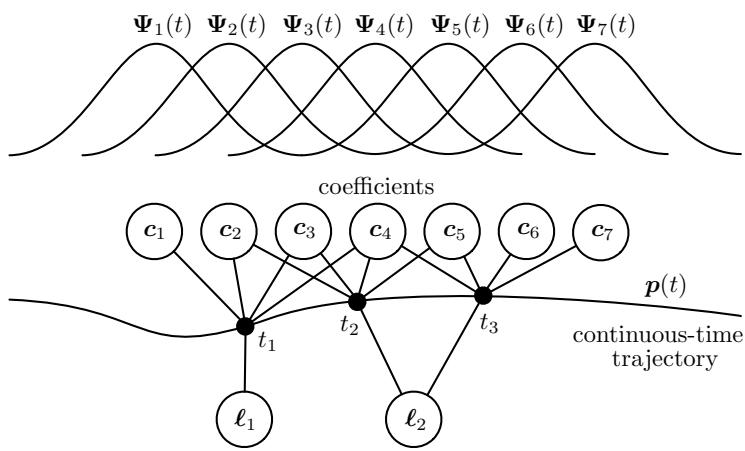
\includegraphics[width=\linewidth]{abdd8e7b3af2c35776787d1be6ccefd148773139241eea52f9e85dbe4af53cf9.jpg}
\caption{图 2.3 用参数化样条表示连续时间轨迹。任意时刻的位姿由具有局部支撑的已知基函数加权求和得到；每个路标测量对应一个连接 4 个系数变量和 1 个路标变量的五元因子，整体因子图仍然非常稀疏。}
\label{fig:abdd8e7b3af2c35776787d1be6ccefd148773139241eea52f9e85dbe4af53cf9}
\end{figure}

代入式（2.36），有

\begin{equation}
\boldsymbol {z} _ {i} = \boldsymbol {h} _ {i} \left(\sum_ {k = 1} ^ {K} \Psi_ {k} (t _ {i}) \boldsymbol {c} _ {k}, \boldsymbol\ell\right) + \boldsymbol {\eta} _ {i}.\tag{2.38}
\end{equation}

如果基函数具有局部支撑，则在 $t_i$ 处只有一小部分系数处于激活状态。令 $\pmb x_i=[\pmb c_i^\top\ \pmb\ell^\top]^\top$ 表示 $t_i$ 处激活的系数变量以及路标变量，就重新得到

\begin{equation}
\boldsymbol {z} _ {i} = \boldsymbol {h} _ {i} (\boldsymbol {x} _ {i}) + \boldsymbol {\eta} _ {i}.\tag{2.39}
\end{equation}

于是可以使用一般方法构造非线性最小二乘问题并进行优化。

如果基函数足够光滑，还可以方便地求取轨迹导数：

\begin{equation}
\dot {\pmb {p}} (t) = \sum_ {k = 1} ^ {K} \dot {\pmb {\Psi}} _ {k} (t) \pmb {c} _ {k}.\tag{2.40}
\end{equation}

这样就能处理依赖速度甚至更高阶导数的传感器输出，而优化变量仍是同一组系数；只需计算基函数的相应导数即可。

通过 MAP 推断求得最优系数后，可以利用式（2.36）或式（2.40）在任意时刻查询轨迹及其导数。如果在推断过程中计算了系数估计的协方差（例如通过求信息矩阵的逆），还可以轻松将其映射为查询位姿或导数的协方差，因为式（2.36）和式（2.40）是线性关系；而基函数的局部支撑意味着只需使用相应的系数边缘协方差。

\subsection{从参数化到非参数化}

基本参数化连续时间方法的主要挑战，是必须决定基函数的类型和数量。基函数太多，容易对测量数据过拟合；太少，又可能没有足够能力表示真实轨迹形状，从而得到过度平滑的解。转向非参数化方法可以部分解决这一问题。

为简化说明，本节暂时假设没有路标变量，只关注位姿变量。采用上一节的参数化方法，线性化最小二乘项（负对数因子）为

\begin{equation}
\left\| \left(\boldsymbol {z} _ {i} - \boldsymbol {h} _ {i} \left(\boldsymbol {x} _ {i} ^ {0}\right)\right) - \boldsymbol {H} _ {i} \boldsymbol {\Psi} _ {i} \delta_ {c, i} \right\| _ {\boldsymbol {\Sigma} _ {i}} ^ {2}.\tag{2.41}
\end{equation}

其中，$\pmb x_i^0$ 是当前解（激活的系数），$\delta_{c,i}$ 是激活系数的更新量，$\Psi_i$ 是在 $t_i$ 处求值并堆叠后的激活基函数，雅可比为

\begin{equation}
\boldsymbol {H} _ {i} = \left. \frac {\partial \boldsymbol {h} _ {i}}{\partial \boldsymbol {x}} \right| _ {\boldsymbol {x} _ {i} ^ {0}}.\tag{2.42}
\end{equation}

像以前一样收集各项，可以写成

\begin{equation}
\boldsymbol {\delta} _ {c} ^ {*} = \underset {\boldsymbol {\delta} _ {c}} {\arg \min} \left(\| \boldsymbol {b} - \boldsymbol {A} \boldsymbol {\Psi} \boldsymbol {\delta} _ {c} \| ^ {2} + \| \boldsymbol {\delta} _ {c} \| ^ {2}\right).\tag{2.43}
\end{equation}

这里加入了正则项 $\|\delta_c\|^2$，倾向于使解的描述长度保持合理，即偏好接近零的样条系数，从而帮助避免过拟合。最优解满足

\begin{equation}
\left(\boldsymbol {\Psi} ^ {\top} \boldsymbol {A} ^ {\top} \boldsymbol {A} \boldsymbol {\Psi} + \mathbf {I}\right) \delta_ {c} ^ {*} = \boldsymbol {\Psi} ^ {\top} \boldsymbol {A} ^ {\top} \boldsymbol {b}.\tag{2.44}
\end{equation}

这可以求得系数的最优更新 $\delta_c^*$。但我们真正关心的是位姿估计，而不是作为中间量的样条系数。测量时刻位姿变量的最优更新为 $\delta^*=\Psi\delta_c^*$。经过简单代数运算，可得

\begin{equation}
\left(\boldsymbol {A} ^ {\mathsf {T}} \boldsymbol {A} + \boldsymbol {K} ^ {- 1}\right) \boldsymbol {\delta} ^ {*} = \boldsymbol {A} ^ {\mathsf {T}} \boldsymbol {b},\tag{2.45}
\end{equation}

这是对式（1.25）正规方程的修改版本。核矩阵 $K=\Psi\Psi^\mathsf T$ 起到正则化或平滑函数的作用。式（2.45）看起来比式（2.44）包含更大的线性系统，因为位姿数量多于样条系数。不过，非参数方法可以利用内置的插值能力，最终减少实际需要求解的系统规模。

为了摆脱显式基函数，可以使用所谓的核技巧，用所选核函数 $\mathcal{K}(t,t')$（例如平方指数核）的计算结果替代基函数的显式内积。构造核矩阵只需要计算基函数内积，因此令 $K=[\mathcal{K}(t_i,t_j)]_{ij}$ 即可。此时不再估计样条的系数（参数），因而称为非参数方法；但仍需调节所选核函数的超参数（例如平方指数核的长度尺度），以实现期望的轨迹平滑程度。由于式（2.45）需要核矩阵的逆，直接这样做似乎代价很高；下一节将说明如何选择核函数，使逆核矩阵非常稀疏。

\subsection{高斯过程}

下面构造一族经过专门设计的核函数，使逆核矩阵及其对应因子图保持稀疏。上一节说明，可以用核函数替换基函数，从而得到非参数连续时间方法；但若直接进行替换，逆核矩阵可能变得稠密。这里从另一条思路出发：图 2.4 给出了一个由本节思想得到的因子图示例，它既保持稀疏，又产生平滑轨迹。

首先选择一个由白噪声驱动的线性时不变随机微分方程（SDE）：\textsuperscript{2}

\begin{equation}
\dot {\boldsymbol {x}} (t) = \boldsymbol {A} \boldsymbol {x} (t) + \boldsymbol {L} \boldsymbol {w} (t),\tag{2.46}
\end{equation}

其中 $\pmb w(t)=\mathcal{GP}(\mathbf0,\pmb{\mathcal{Q}}\delta(t-t'))$ 是零均值白噪声高斯过程，$\pmb{\mathcal{Q}}$ 是功率谱密度矩阵，$\delta(\cdot)$ 是 Dirac delta 函数。该 SDE 将充当运动先验。它可以写出闭式积分解：

\begin{equation}
\boldsymbol {x} (t) = \boldsymbol {\Phi} (t, t _ {1}) \boldsymbol {x} (t _ {1}) + \int_ {t _ {1}} ^ {t} \boldsymbol {\Phi} (t, s) \boldsymbol {L} \boldsymbol {w} (s) d s,\tag{2.47}
\end{equation}

其中 $\Phi(t,s)=\exp(A(t-s))$ 称为转移函数，$t_1$ 是第一次测量的时间戳。若初始状态均值为零，则后续状态均值也保持为零；状态的协方差函数（即核函数）为

\begin{equation}
\boldsymbol {\mathcal {K}} (t, t') = \boldsymbol {\Phi} (t, t _ {1}) \boldsymbol {\mathcal {K}} (t _ {1}, t _ {1}) \boldsymbol {\Phi} (t', t _ {1}) ^ {\top} + \int_ {t _ {1}} ^ {\min (t, t')} \boldsymbol {\Phi} (t, s) \boldsymbol {L} \boldsymbol {\mathcal{Q}} \boldsymbol {L} ^ {\top} \boldsymbol {\Phi} (t', s) ^ {\top} d s.\tag{2.48}
\end{equation}

在全部测量时刻计算核函数并构造核矩阵时，可以利用简洁关系

\begin{equation}
\boldsymbol {K} = \boldsymbol {\Phi} \boldsymbol {Q} \boldsymbol {\Phi} ^ {\mathsf T},\tag{2.49}
\end{equation}

其中 $Q=\operatorname{diag}(\mathcal{K}(t_1,t_1),Q_1,\ldots,Q_M)$，且

\begin{equation}
\boldsymbol {\Phi} = \left[ \begin{array}{c c c c c} \mathbf {I} & & & & \\ \boldsymbol {\Phi} (t _ {2}, t _ {1}) & \mathbf {I} & & & \\ \boldsymbol {\Phi} (t _ {3}, t _ {1}) & \boldsymbol {\Phi} (t _ {3}, t _ {2}) & \mathbf {I} & & \\ \vdots & \vdots & \vdots & \ddots & \\ \boldsymbol {\Phi} (t _ {M}, t _ {1}) & \boldsymbol {\Phi} (t _ {M}, t _ {2}) & \cdots & \boldsymbol {\Phi} (t _ {M}, t _ {M-1}) & \mathbf {I} \end{array} \right].\tag{2.50}
\end{equation}

其中

\begin{equation*}
Q_i=\int_{t_{i-1}}^{t_i}\Phi(t_i,s)L\mathcal{Q}L^\top\Phi(t_i,s)^\top ds.
\end{equation*}

矩阵 $\Phi$ 是由各时间点之间的转移函数构成的下三角块矩阵，其对角块为单位阵。由于我们需要的是逆核矩阵，$K^{-1}=\Phi^{-\top}Q^{-1}\Phi^{-1}$；而 $Q$ 是块对角矩阵，逆可以逐个对角块计算。更重要的是，$\Phi^{-1}$ 只有主块对角线和紧邻其下的一个块对角线非零：

\begin{equation}
\boldsymbol {\Phi} ^ {- 1} = \left[ \begin{array}{c c c c c c} \mathbf {I} & & & & & \\ - \boldsymbol {\Phi} (t _ {2}, t _ {1}) & \mathbf {I} & & & & \\ & - \boldsymbol {\Phi} (t _ {3}, t _ {2}) & \mathbf {I} & & & \\ & & - \boldsymbol {\Phi} (t _ {4}, t _ {3}) & \ddots & & \\ & & & \ddots & \mathbf {I} \\ & & & & - \boldsymbol {\Phi} (t _ {M}, t _ {M - 1}) & \mathbf {I} \end{array} \right].\tag{2.51}
\end{equation}

因此，任意长度轨迹的逆核矩阵 $K^{-1}$ 都是块三对角的。根据前面对因子图的讨论，式（2.45）左端的稀疏性与因子图结构密切相关；这里 $K^{-1}$ 作为整条轨迹的运动先验，可以用非常稀疏的因子图表示。

$K^{-1}$ 之所以具有这种稀疏因子图，是因为出发点 SDE 的状态具有马尔可夫性。实际含义是：根据式（2.46）想表达的运动先验，状态可能需要包含更高阶量，而不只是位姿，还包括其导数。例如，若希望采用“恒速”先验，可以选择

\begin{equation}
\underbrace {\left[ \begin{array}{c} \dot {\boldsymbol {p}} (t) \\ \dot {\boldsymbol {v}} (t) \end{array} \right]} _ {\dot {\boldsymbol {x}} (t)} = \underbrace {\left[ \begin{array}{c c} \mathbf {0} & \mathbf {I} \\ \mathbf {0} & \mathbf {0} \end{array} \right]} _ {\boldsymbol {A}} \underbrace {\left[ \begin{array}{c} \boldsymbol {p} (t) \\ \boldsymbol {v} (t) \end{array} \right]} _ {\boldsymbol {x} (t)} + \underbrace {\left[ \begin{array}{c} \mathbf {0} \\ \mathbf {I} \end{array} \right]} _ {\boldsymbol {L}} \boldsymbol {w} (t).\tag{2.52}
\end{equation}

这里的状态包含位姿及其导数。这种使用增广状态的形式有时称为同时轨迹估计与建图（STEAM），是 SLAM 的一种变体。

上述连续时间轨迹估计实际上是高斯过程回归 \textsuperscript{[909]} 的一个例子。建立这一联系后，在测量时刻求解状态，就可以利用 GP 插值在其他时刻查询轨迹的均值和协方差。采用稀疏核方法时，每次查询的代价相对于测量数量 $M$ 为常数，因为只涉及夹住查询时刻的两个估计状态。

还可以利用 GP 插值减少所需控制点的数量，不必在每个测量时刻都设置控制点，这类似于 GP 的诱导点思想。例如，每次激光扫描设置一个控制点，但仍使用扫描过程中每个点的独立时间戳。这样，测量时刻、估计时刻和查询时刻可以彼此不同。GP 的核还提供了适当的正则化，因此无需担心设置过多估计时刻导致过拟合，但仍需有足够的估计时刻来捕捉轨迹细节。

\subsection{Lie 群上的样条与高斯过程}

当状态位于流形上时，同样可以使用样条和 GP 连续时间方法。若流形是 Lie 群，两种方法都利用 Lie 代数，但方式不同。下面先介绍样条，再介绍高斯过程。

\subsubsection{Lie 群上的样条}

使样条适用于 Lie 群的关键，是采用累积形式。对于向量空间，假设所有自由度使用相同基函数，式（2.36）可简化为

\begin{equation}
\boldsymbol {p} (t) = \sum_ {k = 1} ^ {K} \psi_ {k} (t) \boldsymbol {p} _ {k},\tag{2.53}
\end{equation}

其中 $\pmb p_k$ 是样条控制点，$\psi_k(t)$ 是标量基函数。将其改写为累积形式：

\begin{equation}
\boldsymbol {p} (t) = \psi_ {1} ^ {c} (t) \boldsymbol {p} _ {1} + \sum_ {k = 2} ^ {K} \psi_ {k} ^ {c} (t) \left(\boldsymbol {p} _ {k} - \boldsymbol {p} _ {k - 1}\right),\tag{2.54}
\end{equation}

其中累积基函数为

\begin{equation}
\psi_ {k} ^ {c} (t) = \sum_ {\ell = k} ^ {K} \psi_ {\ell} (t).\tag{2.55}
\end{equation}

例如，对时间间隔均匀为 $T$ 的线性插值，定义 $\alpha_k(t)=(t-(k-1)T)/T$，普通基函数为

\begin{equation}
\psi_1(t)=\begin{cases}1-\alpha_1(t),&0\le t<T\\0,&\text{其他情况},\end{cases}\quad
\psi_K(t)=\begin{cases}\alpha_K(t),&(K-1)T\le t<KT\\0,&\text{其他情况},\end{cases}\tag{2.56}
\end{equation}

而对 $k=2,\ldots,K-1$，

\begin{equation}
\psi_k(t)=\begin{cases}\alpha_{k-1}(t),&(k-2)T\le t<(k-1)T\\1-\alpha_k(t),&(k-1)T\le t<kT\\0,&\text{其他情况}.
\end{cases}\tag{2.57}
\end{equation}

对应的累积基函数为

\begin{equation}
\psi_1^c(t)=1,\qquad \psi_K^c(t)=\begin{cases}0,&t<(K-1)T\\\alpha_K(t),&(K-1)T\le t,\end{cases}\tag{2.58}
\end{equation}

以及对 $k=2,\ldots,K-1$，

\begin{equation}
\psi_k^c(t)=\begin{cases}0,&t<(k-1)T\\\alpha_k(t),&(k-1)T\le t<kT\\1,&kT\le t.
\end{cases}\tag{2.59}
\end{equation}

图 2.5 展示了这些基函数的形状。

累积基函数的主要优点是：在给定时间戳处，大多数基函数都不激活。对于线性样条，当 $(k-1)T\le t<kT$ 时，

\begin{equation}
\boldsymbol {p} (t) = \boldsymbol {p} _ {k - 1} + \psi_ {k} ^{c} (t) (\boldsymbol {p} _ {k} - \boldsymbol {p} _ {k - 1}).\tag{2.60}
\end{equation}

此时只需计算一个基函数；更高阶样条在任意时刻也只会有少量激活基函数。

在 Lie 群上使用样条时，用 Lie 群运算（矩阵乘法）替代累积表达式中的加法。以线性样条为例，在 $(k-1)T\le t<kT$ 时，$\operatorname{SE}(d)$ 中的元素可以写成

\begin{equation}
\boldsymbol {T} (t) = \mathrm{Exp} \left(\psi_ {k} ^ {c} (t) \mathrm{Log} \left(\boldsymbol {T} _ {k} \boldsymbol {T} _ {k - 1} ^ {- 1}\right)\right) \boldsymbol {T} _ {k - 1}.\tag{2.61}
\end{equation}

这里选择了左侧扰动，当然也可以采用右侧扰动。将 $\pmb T(t_i)$ 代入任意测量表达式，在控制点 $\pmb T_k$ 的 Lie 代数扰动上进行线性化，即可用于 MAP 框架。由于基函数具有紧支撑，在一个测量时刻只有少量控制点激活。

对于线性样条，式（2.61）可写为

\begin{equation}
\boldsymbol {T} (t) = \left(\boldsymbol {T} _ {k} \boldsymbol {T} _ {k - 1} ^ {- 1}\right) ^ {\alpha_ {k} (t)} \boldsymbol {T} _ {k - 1}.\tag{2.62}
\end{equation}

对 $\pmb T(t)$ 中的表达式进行线性化时，分别扰动两个控制位姿，使

\begin{equation}
\operatorname{Exp} (\boldsymbol {\xi} (t)) \boldsymbol {T} ^ {0} (t) = \left(\operatorname{Exp} (\boldsymbol {\xi} _ {k}) \boldsymbol {T} _ {k} ^ {0} \boldsymbol {T} _ {k - 1} ^ {0^{-1}} \operatorname{Exp} (- \boldsymbol {\xi} _ {k - 1})\right) ^ {\alpha_ {k} (t)} \operatorname{Exp} (\boldsymbol {\xi} _ {k - 1}) \boldsymbol {T} _ {k - 1} ^ {0}.\tag{2.63}
\end{equation}

插值位姿扰动 $\pmb\xi(t)$ 与两个控制点扰动 $\pmb\xi_k$、$\pmb\xi_{k-1}$ 的关系可近似为

\begin{equation}
\boldsymbol {\xi} (t) \approx (\boldsymbol {I} - \boldsymbol {A} (\alpha_ {k} (t))) \boldsymbol {\xi} _ {k - 1} + \boldsymbol {A} (\alpha_ {k} (t)) \boldsymbol {\xi} _ {k},\tag{2.64}
\end{equation}

其中

\begin{equation}
\boldsymbol {A} \left(\alpha_ {k} (t)\right) = \alpha_ {k} (t) \boldsymbol {J} \left(\alpha_ {k} (t) \boldsymbol {T} _ {k} ^ {0} \boldsymbol {T} _ {k - 1} ^ {0^{-1}}\right) \boldsymbol {J} \left(\boldsymbol {T} _ {k} ^ {0} \boldsymbol {T} _ {k - 1} ^ {0^{-1}}\right) ^ {- 1}.\tag{2.65}
\end{equation}

这里 $J(\cdot)$ 是 $\operatorname{SE}(d)$ 的左雅可比。利用式（2.64），即可将测量时刻位姿的变化与两侧控制点位姿关联起来，形成用于 MAP 估计的线性化误差。例如，式（2.16）的线性化测量模型可写成

\begin{equation}
\boldsymbol {e} _ {i} (t) \approx \boldsymbol {z} _ {i} - \boldsymbol {h} _ {i} \left(\boldsymbol {T} ^ {0} (t) \tilde {\ell} _ {i}\right) - \boldsymbol {H} _ {i} \boldsymbol {\xi} (t).\tag{2.66}
\end{equation}

将式（2.64）代入即可得到关于两侧控制点的线性化误差：

\begin{equation}
\pmb {e} _ {i} (t) \approx \pmb {z} _ {i} - \pmb {h} _ {i} \left(\pmb {T} ^ {0} (t) \tilde {\pmb {\ell}} _ {i}\right) - \pmb {H} _ {i} \left(\pmb {I} - \pmb {A} (\alpha _ {k} (t))\right) \pmb {\xi} _ {k - 1} - \pmb {H} _ {i} \pmb {A} (\alpha _ {k} (t)) \pmb {\xi} _ {k}.\tag{2.67}
\end{equation}

其中还需将 $t$ 时刻的名义位姿 $\pmb T^0(t)=(\pmb T_k^0\pmb T_{k-1}^{0^{-1}})^{\alpha_k(t)}\pmb T_{k-1}^0$ 代入 $h_i$ 和 $H_i$。这相当于沿线性样条链式传播导数；高阶样条也可以采用同样过程。

\subsubsection{Lie 群上的高斯过程}

在 Lie 群上使用高斯过程时，同样利用 Lie 代数。图 2.6 展示了相应的 GP 运动先验因子。根据所选运动先验，控制点状态也可以包含额外的轨迹导数。

我们在一组控制点状态之间使用局部 GP，这与样条类似。对 $\operatorname{SE}(d)$，定义控制点之间的局部变量 $\pmb\xi_k(t)$。例如，对 $\operatorname{SE}(d)$ 的“随机游走”先验，可以选择

\begin{equation}
\dot {\pmb {\xi}} _ {k} (t) = \pmb {w} (t), \quad \pmb {w} (t) = \mathcal {GP} (\pmb {0}, \pmb {\mathcal {Q}} \delta (t - t ^ {\prime})),\tag{2.68}
\end{equation}

这里的变量定义在控制点 $\pmb T_k$ 和 $\pmb T_{k+1}$ 之间。该 SDE 的转移函数为单位阵，随机积分得到

\begin{equation}
\boldsymbol {\xi} _ {k} (t) = \underbrace {\boldsymbol {\xi} _ {k} (t _ {k})} _ {\mathbf {0}} + \int_ {t _ {k}} ^ {t} \boldsymbol {w} (s) d s,\tag{2.69}
\end{equation}

于是运动先验为

\begin{equation}
\boldsymbol {\xi} _ {k} (t) \sim \mathcal {GP} (\mathbf {0}, \min (t, t ^ {\prime}) \boldsymbol {\mathcal {Q}}).\tag{2.70}
\end{equation}

若控制点每隔 $T$ 秒均匀分布，则逆核矩阵为 $\kappa^{-1}=\Phi^{-\top}Q^{-1}\Phi^{-1}$，其中

\begin{equation}
\boldsymbol {\Phi} ^ {- 1} = \left[ \begin{array}{c c c c} \mathbf {I} & & & \\ - \mathbf {I} & \mathbf {I} & & \\ & \ddots & \ddots & \\ & & - \mathbf {I} & \mathbf {I} \end{array} \right], \quad \boldsymbol {Q} = \operatorname{diag} \left(\boldsymbol {\mathcal {K}} (t _ {1}, t _ {1}), T \boldsymbol {\mathcal {Q}}, \ldots , T \boldsymbol {\mathcal {Q}}\right).\tag{2.71}
\end{equation}

局部变量下的误差为

\begin{equation}
\boldsymbol {e} _ {k} = \left\{ \begin{array}{l l} \mathrm{Log} (\boldsymbol {T} _ {1} \check {\boldsymbol {T}} _ {1} ^ {- 1}) & k = 1 \\ \boldsymbol {\xi} _ {k - 1} (t _ {k}) - \boldsymbol {\xi} _ {k - 1} (t _ {k - 1}) & k > 1 \end{array} \right.,\tag{2.72}
\end{equation}

其中 $\check{\pmb T}_1$ 是初始位姿先验。用全局变量表示时，同一误差为

\begin{equation}
\boldsymbol {e} _ {k} = \left\{ \begin{array}{l l} \operatorname{Log} \left(\boldsymbol {T} _ {1} \check {\boldsymbol {T}} _ {1} ^ {- 1}\right) & k = 1 \\ \operatorname{Log} \left(\boldsymbol {T} _ {k} \boldsymbol {T} _ {k - 1} ^ {- 1}\right) & k > 1 \end{array} \right..\tag{2.73}
\end{equation}

图 2.6 给出了这种随机游走 GP 运动先验的因子图。与线性样条类似，若要在其他时刻查询轨迹，可以使用 GP 插值；对于随机游走先验，结果再次是线性插值：

\begin{equation}
\pmb {T} (t) = \left(\pmb {T} _ {k} \pmb {T} _ {k - 1} ^ {- 1}\right) ^ {\alpha_ {k} (t)} \pmb {T} _ {k - 1},\tag{2.74}
\end{equation}

其中 $\alpha_k(t)=(t-(k-1)T)/T$，且 $(k-1)T\le t<kT$。与样条方法不同，这里的线性插值是 SDE 选择的间接结果，而不是显式指定的形式；如果一开始选择高阶 SDE，就会得到高阶插值样条。

最后，需要将误差项线性化以用于 MAP 估计。再次利用 Lie 群扰动方法，对于式（2.73）的第二种情形，有

\begin{equation}
\begin{array}{c} \boldsymbol {e} _ {k} = \operatorname{Log} \left(\operatorname{Exp} (\boldsymbol {\xi} _ {k}) \boldsymbol {T} _ {k} ^ {0} \boldsymbol {T} _ {k - 1} ^ {0^{-1}} \operatorname{Exp} (- \boldsymbol {\xi} _ {k - 1})\right) \\ \approx \operatorname{Log} \left(\boldsymbol {T} _ {k} ^ {0} \boldsymbol {T} _ {k - 1} ^ {0^{-1}}\right) + \boldsymbol {\xi} _ {k} - \operatorname{Ad} \left(\boldsymbol {T} _ {k} ^ {0} \boldsymbol {T} _ {k - 1} ^ {0^{-1}}\right) \boldsymbol {\xi} _ {k - 1}, \end{array}\tag{2.75}
\end{equation}

其中 $\pmb T_k^0$ 和 $\pmb T_{k-1}^0$ 是当前猜测，$\pmb\xi_k$ 和 $\pmb\xi_{k-1}$ 是待求扰动，$\operatorname{Ad}(\cdot)$ 是 $\operatorname{SE}(d)$ 的伴随表示。式（2.75）的线性化形式可以在每次迭代中直接纳入标准 MAP 估计框架。

此外，若想利用式（2.74）减少随机游走示例中的控制点数量，可以采用式（2.67）中针对线性样条的同一方法，因为两者最终都归结为 Lie 群控制点之间的线性插值。样条与 GP 的根本区别在于：GP 方法使用运动先验项（见图 2.6）对问题进行正则化，而样条方法不使用这种先验。\textsuperscript{4}

\section{延伸阅读与近期趋势}

关于流形，尤其是 Lie 群上的估计，已有大量研究。机器人领域的奠基性参考是 Chirikjian \textsuperscript{[205]} 及 Chirikjian 和 Kyatkin \textsuperscript{[207]}；这些著作理论基础扎实，并给出了处理流形不确定性的通用工具，包括全局不确定性。关于流形优化，Boumal \textsuperscript{[106]} 是面向机器人应用的优秀参考。Barfoot \textsuperscript{[47]} 更详细地讨论了不确定性仍较为集中的 Lie 群估计，这与本章内容相近。连续时间估计方面，Talbot 等人 \textsuperscript{[1067]} 提供了参数化和非参数化方法的综合综述；Barfoot \textsuperscript{[47]} 也对非参数方法作了较为详细的说明。

与上一章类似，离群点处理、使算法可微，以及利用本章工具支持不同类型的传感器等近期趋势，将在后续章节中进一步讨论。


\backmatter
\chapter*{后续章节}
本项目的目录和构建脚本支持继续添加后续章节的中文翻译。

\end{document}
